%!TEX root = ../thesis.tex
\chapter{The Pleiades as a benchmark}
\label{chap:pleiades}

\section{Generalities}
\label{sect:generalities}
The ancient greeks named Pleiades to a crowded group of nine stars which they believed shared a common origin. These stars were the seven sisters, that together with their parents the titan Atlas and the nymph Pleione, were put in the sky  by the god Zeus.
 
Today, we call the Pleiades cluster not just to the nine stars that made up the original Pleione family, but to a much larger group, which according to \citet{Bouy2015} adds up to $\sim2100$ members. This cluster is fairly close to the sun, $\sim 134$ pc \cite[with parallaxes of $7.44\pm0.08$ and $7.48\pm0.03$ according to][respectively]{Galli2017,2017A&A...601A..19G}, and is also young in galactic scales, with only $\sim125$ \gls{myr} \citep{Stauffer1998}. Since it is located in the solar neighbourhood, it has a distinctive angular velocity in the plane of the sky: about $-16\,\mathrm{mas\cdot yr^{-1}}$ in right ascension and $20\,\mathrm{mas\cdot yr^{-1}}$ in declination. It has a metallicity near to the solar one \cite[{[Fe/H]$\sim$0},][]{Takeda2017}. Also, it has an almost null extinction of $A_v=0.12$ mag \citep{Guthrie1987}. These properties make the Pleiades one of the most studied clusters in the history of astronomy \footnote{Probably just after the Orion complex.}. Thus making it also the perfect test case of the methodology developed in this work.

As stated in the previous Chapter,  the objective of the present study is to obtain the statistical distributions of the distance, position, velocity, luminosity and mass of the Pleiades cluster. Thus, in the following sections I will describe the current knowledge of the Pleiades, concerning these astrophysical quantities. 
 
\section{The distance to the Pleiades}

\subsection{Measuring distances}
In astronomy, measuring distances is a complicated task. Techniques vary according to the distance scale that they aim to measure. The distance ladder is constructed from smaller to larger distances. The first step in this ladder is the distance to the sun. After that, the distance to the planets and then to the stars. This works deals only with nearby clusters, thus I only focus on measuring distances to these objects. 

The most direct way to measure distance to nearby stars is by means of the trigonometric parallax. This is the maximum relative angular displacement, with respect to the far distant stars, that an object suffers in the course of a year. {It is usually reported in miliarc seconds (mas)}. The relative displacement results from the movement of the Earth (thus of the observer) on its orbit around the sun. The relative displacement is maximal when measurements are taken at opposed points in the earth's orbit, when they are separated by six months. If the parallax were measured in seconds of arc and with infinite precision, then the distance to the object would be obtained by simply inverting its parallax. By doing so, the distance will be measured in parsecs. This unit gets its name from parallax-second. Thus an object located at a distance of one parsec from the sun shows a parallax of one arc second. The further the object is, the smaller the parallax gets.

As any measurement, parallaxes have uncertainties, which usually represent, or are a proxy for, the width of the distribution. {The parallax distribution is also continuous and non-limited}. 

When transforming parallaxes into distances we may be tempted to take a summary of the distribution, the mean for example, and just invert it to obtain the distance. This only holds if the summary corresponds to the true value (i.e. the statistic is unbiased). {The true value is that which would be observed in the presence of negligible uncertainties}. However, because measurements have uncertainties, which almost always are not negligible, the inversion of the parallax not always renders an unbiased estimate of the distance. {Assuming that the distribution of parallax measurements of an object is Gaussian, \citet{Lutz1973} found that the distance to the object can be reasonably recovered by just inverting the parallax if its relative uncertainty is below 0.15-0.20. However, the shape of the distribution of parallax measurements of an object (the second and higher order moments) plays also an important role. Transforming the parallax distribution into that of the distance require more than a simple inversion.}  

Several authors have proposed different approaches to the problem of distance determination using parallaxes, see for example \citet{Lutz1973,2015PASP..127..994B,2016ApJ...832..137A,2016ApJ...833..119A}. The proper way, as \citet{2015PASP..127..994B} points out, consists of inferring the true distances given the observed parallaxes. For that, a prior on the distance must be established. The authors mentioned before describe three different kinds of priors and the methodology needed to infer the true distances. However, going into deeper detail is beyond the scope of this work.

Now, I focus on the particular case of the distance to the Pleiades. One of the first measurements of the Pleiades distance using parallaxes was done by \citet{1999A&A...341L..71V} using \emph{Hipparcos} data.{ Later, the same author \citep{2009A&A...497..209V} refined his analysis and obtained a value of $120\pm1.9$ pc. However, \citet{2000ApJ...533..938G} with parallax measurements of seven stars taken at the Allegheny Observatory, and later \citet{2005AJ....129.1616S} with the parallaxes of three stars measured with the Fine Guidance Sensors of the \emph{Hubble Space Telescope}, derived distances of $130.9\pm7.4$ pc and $134.6\pm3.1$ pc, respectively. Finally, \citet{2014Sci...345.1029M} using very long baseline radio interferometric parallaxes of three stars obtained a distance of $136.2\pm1.2$ pc.} There was a clear controversy between \emph{Hipparcos} data and other parallax measurements. The current data release of the \gls{tgas}, gives a distance to the Pleiades of $133.7\pm0.5$ pc \cite[from a parallax of $7.48\pm0.03$ mas][]{2017A&A...601A..19G}. This seems to indicate that the \emph{Hipparcos} parallaxes were somehow biased.

Our research group finds a distance to the Pleiades of $134.4^{+2.9}_{-2.8} $ pc (from a parallax of $7.44\pm0.08$ mas) \citep{Galli2017}, which is in good agreement with the one of \gls{tgas}. We found this distance using the kinematic parallaxes delivered by the moving cluster technique. This essentially exploits the fact that since clusters are bound, their members show a clear kinematic footprint: they seem to converge to a point in the sky \citep{1964IAUS...20...50B}. Using this point and the velocity of the members (proper motion and radial velocities) it is possible to derive individual parallaxes. Furthermore, these individual parallaxes show a distribution which results from the dispersion of the cluster members distances along the line of sight. Figures \ref{fig:parallaxPhillip} and \ref{fig:parallaxTGAS} show the distribution of parallaxes for the Pleiades candidate members according to \citet{Galli2017} and \citet{2017A&A...601A..19G}, respectively. As can be seen from these Figures, the results of both works agree on the mean of the parallax distribution. However, they recover different variances. This difference results from the discrepancy in the number of objects, 1210 in \citet{Galli2017} vs. 152 in \citet{2017A&A...601A..19G}, and in the selection function of the two surveys. The \gls{tgas} sample is limited to the bright objects ($V \sim 11.5$ mag), whereas the \gls{ddr2} includes the faint end of the distribution ($i\sim25$ mag). For these reasons, in the following I adopt the distance found by \citet{Galli2017}.

Nevertheless, the distance distribution {(measured uncertainties comprised)} is only the depth component of the space distribution of the cluster, the other two components are given by the projected spatial distribution. 

\begin{figure}[ht!]
    \centering
    \begin{subfigure}[t]{\textwidth}
    \centering
        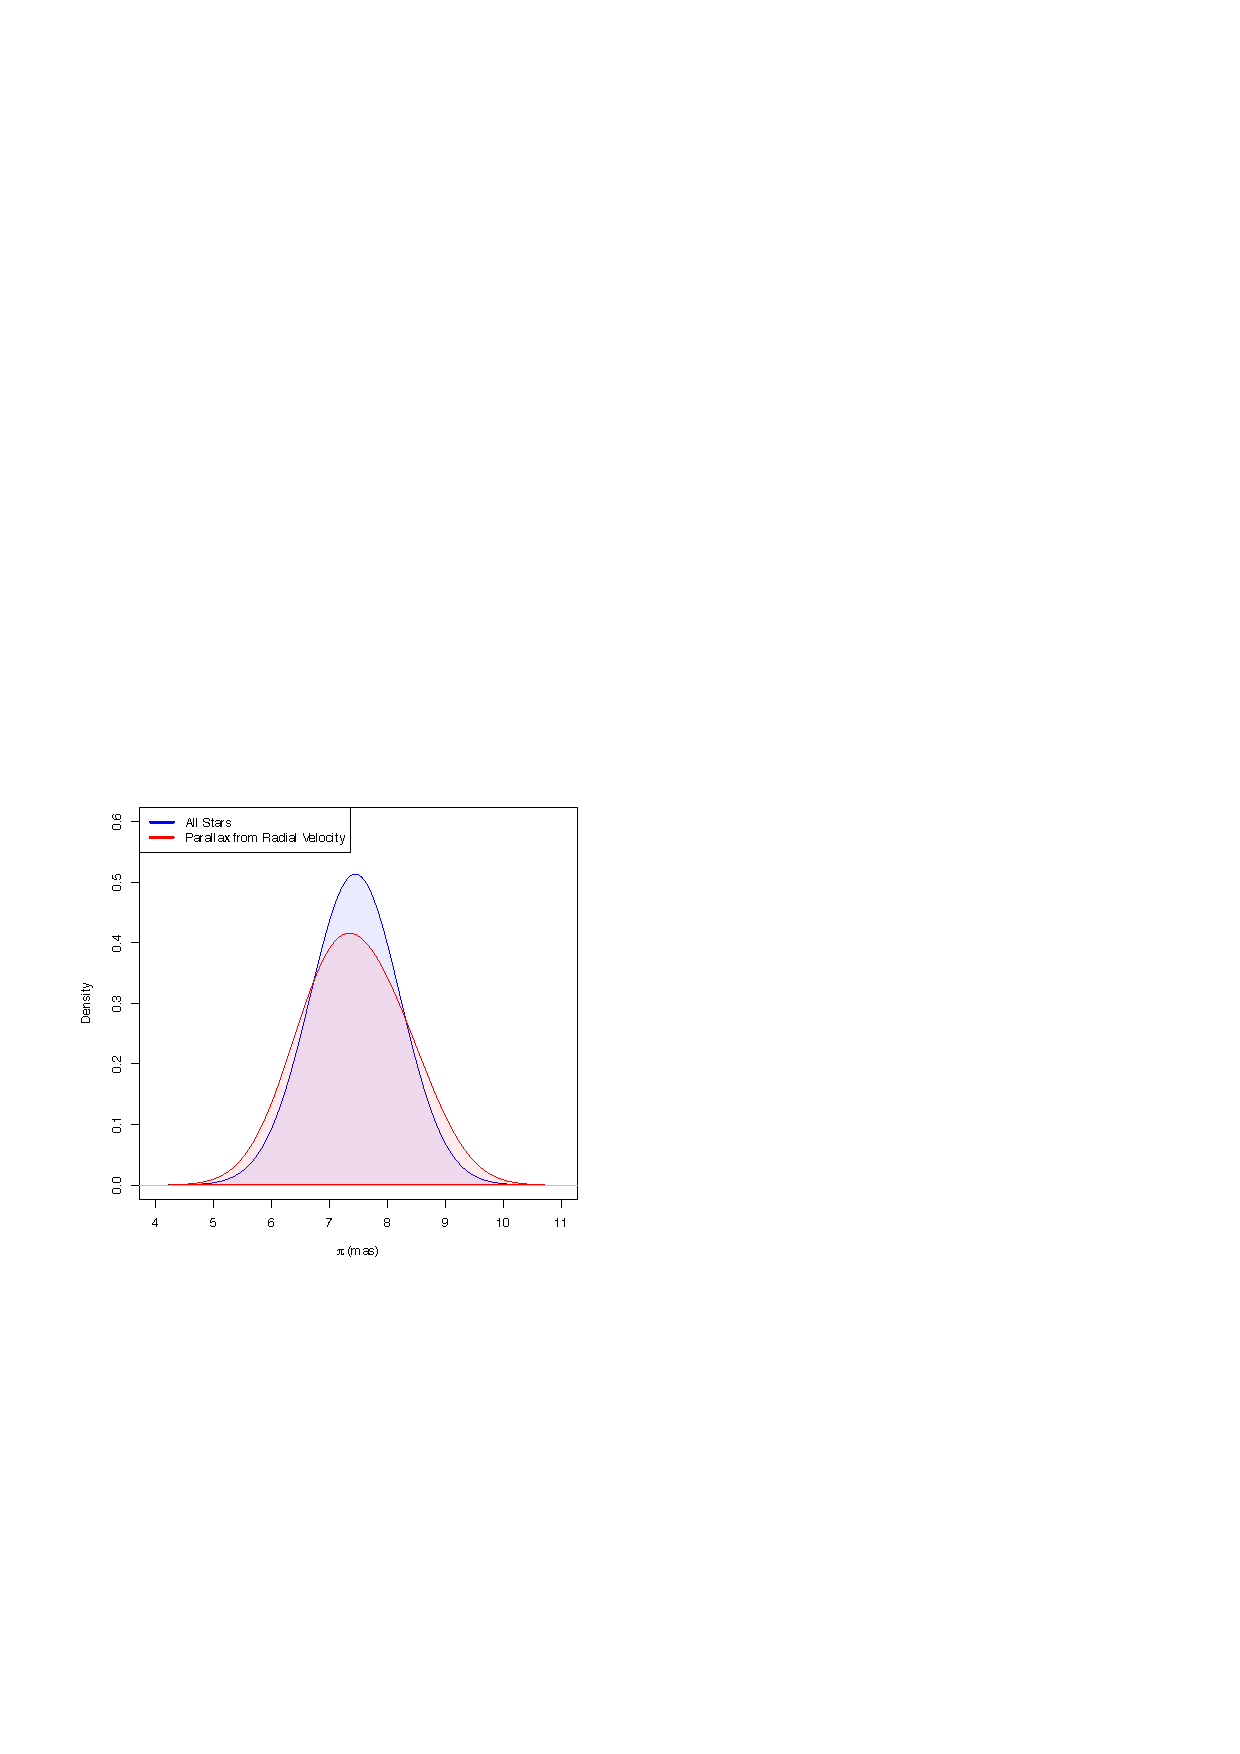
\includegraphics[height=8cm]{background/Figures/F13_Galli2017.pdf}
        \caption{Parallaxes according to \citet{Galli2017}. The red line shows all their candidate members (1210) while the blue one only those with known radial velocity (64). Reproduced from Figure 13 of \citet{Galli2017}, \textit{\usebibentry{Galli2017}{Title}}, \usebibentry{Galli2017}{Journal}, Vol. \usebibentry{Galli2017}{Volume}.}
        \label{fig:parallaxPhillip}
    \end{subfigure}
    \begin{subfigure}[t]{\textwidth}
    \centering
       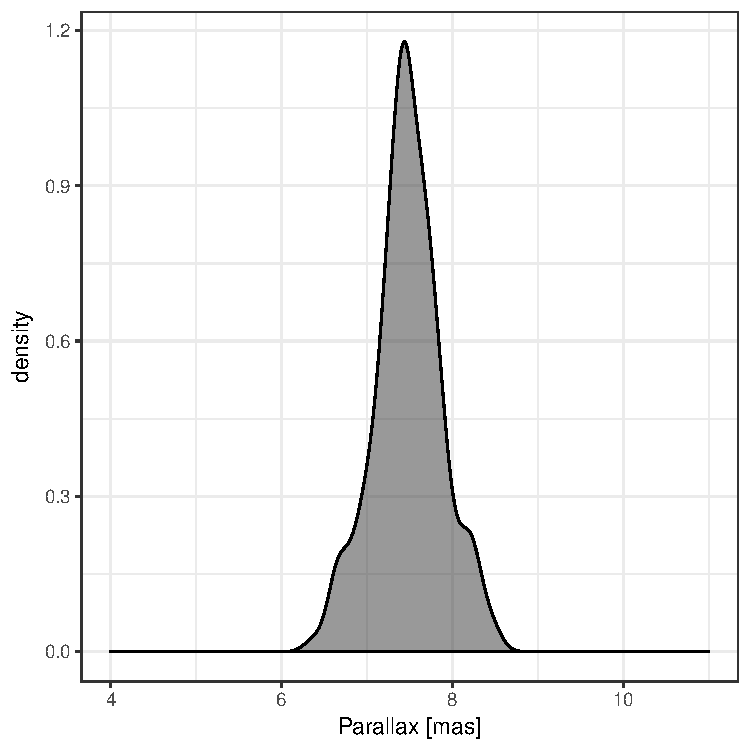
\includegraphics[height=8cm]{background/Figures/Parallax_GaiaCol2017.pdf}
        \caption{Parallaxes according to \citet{2017A&A...601A..19G}. Only their 152 candidate members.}
        \label{fig:parallaxTGAS} 
    \end{subfigure}
    \caption{Distribution of parallaxes for the Pleiades members.}
\end{figure}



\section{Projected spatial distribution}
\label{sect:PSD}
The \gls{psd} is the two dimensional projection, in the plane of the sky (the one perpendicular to the line of sight), of the cluster three dimensional space distribution. In astronomy, object positions are commonly measured in what is called the Equatorial Coordinate System\footnote{Another common coordinate system is the Alt-Azimuth one \cite[see][]{Smart1977}.}. It can be thought as the projection of the geographical coordinates, latitude and longitude, into the sky. The Right Ascension (R.A.) coordinate, analogous to the longitude, gives the objects angle with the vernal equinox, in an eastward direction and along the celestial equator. The Declination (Dec.) coordinate, analogous to the latitude, gives the object angle perpendicular to the celestial equator, positive to the North and negative to the South. For more details of the Equatorial Coordinate System see for example \citet{Smart1977}. 

{Stellar positions of an object are far more easily measured than its parallax. For this reason, just a small fraction of objects with stellar positions has also parallax measurements. In the case of the Pleiades, after cross-matching the \emph{Hipparcos} catalogue \citep{1997A&A...323L..49P} with the candidate members of \citet{Bouy2015}, I find that only 70 of the $\sim2100$ candidates have parallaxes. As seen in the previous section, this figure is roughly doubled with the new \gls{tgas} \citep{2016A&A...595A...1G} data release. In addition to the scarcity of parallaxes, which is expected to be solved with future \emph{Gaia} data releases, the relative uncertainties in R.A. and Dec. coordinates, measured in degrees, are far better ($\sim 10^{-5}$) than those of the parallaxes ($\sim10^{-1}$), measured in mas. Transforming these relative precisions into parsecs, by means of the distance, it is seen that the position in the plane of the sky is $10^4$ more precise than along the line of sight.  These two are the main reasons, for which the Pleiades space distribution has been studied mainly through its \gls{psd}. The latter has been the subject of several studies. }

One of the earliest results of the Pleiades \gls{psd} was done by \citet{Limber1962}. He used a mixture of four indices polytropic distribution, as was described is his earlier \citet{Limber1961} work, to fit the \gls{psd} of the 246 candidate members of \citet{Trumpler1921}. These candidates were contained in a $3^{\circ}$ radius around \emph{Alcyone} (one of the central most massive stars of the Pleiades cluster). 

\sloppy
Later, \citet{Pinfield1998} fitted King profiles \citep{King1962} to candidate members from the literature, which were contained in a $3^{\circ}$ radius area. They fitted King profiles to objects within different mass ranges, their bins centred at $5.2,1.65,0.83$ and $0.3 \,\mathrm{M_{\odot}}$. The tidal radius they found, $13.1\,pc$ ($\sim 5.6^{\circ}$) contained $1194$ candidate members. The total mass of these members amounted to $735\,\mathrm{M_{\odot}}$. These authors also estimated a mean individual stellar mass of $0.616\,\mathrm{M_{\odot}}$. {They measured core radius in the 0.9 to 2.91 pc range for the King profiles fitted to their different mass bins.}

On the same year \citet{Raboud1998} also fitted a King's profile \citep{King1962} to a list of 270 candidate members with masses in the range $0.74-7.04\,\mathrm{M_{\odot}}$, which were contained within a $5^{\circ}$ radius area. They found a core radius of $1.5$ pc and a tidal radius of $17.5$ pc ($7.5$ degrees). Using different approaches, they derived a total mass within the range of $500 -8000 \,\mathrm{M_{\odot}}$. They also measured an ellipticity of $\epsilon=0.17$, however they did not make any explicit mention on the position angle of the axis of the ellipse.

Later, \citet{Adams2001} also fitted a King profile to objects with membership probabilities $p>0.3$ within a radius of $10^{\circ}$. They found a core radius of $2.35-3.0$ pc and a tidal radius of $13.6-16$ pc ($5.8 - 6.8^{\circ}$). They estimate a total mass of $\sim 800\,\mathrm{M_{\odot}}$, and their measured ellipticities are in the range $0.1-0.35$. 

\citet{Converse2008} fit a King profile to a sample of 1245 candidate members from \citet{Stauffer2007} compilation. These objects have masses greater than $0.08\,\mathrm{M_{\odot}}$ and are contained within a $5^{\circ}$ radius. They obtained a tidal radius of $18$ pc (7.7 degrees) and a core radius of  $1.3$ pc. Later, \citet{Converse2010} refined their study and obtained a core radius of $2.0\pm0.1$ pc, a tidal radius of $19.5 \pm 1.0 $ pc ($\sim 8.3$ degrees) and a total mass of $870\pm35\,\mathrm{M_{\odot}}$. In Fig. \ref{fig:spatialConverse}, I reproduce the surface density fit obtained by these authors.

The previous summary of results shows at least two interesting points. In the first place, King profile \citep{King1962} has been the preferred choice for the Pleiades cluster, although it was created to fit the \gls{psd} of globular clusters. Since globular clusters are farther away than open clusters and in a low density environment, usually the end of their \gls{psd} is well within the survey area. The second point concerns the increasing trend of the tidal radius with the size of the survey and the publication date, see Table \ref{tab:tidal_iterature}. As the surveys increase in area the derived tidal radii increase as well. The exception is the work of \citet{Adams2001}. Since these authors used low membership probability ($\geq0.3$) objects, they may have also fitted the field. The surface density of a tidally truncated cluster should diminish with radius and eventually go to zero at the tidal radius. However, as can be seen in Figure \ref{fig:spatialAdams}, where I reproduce Figure 8 of \citet{Adams2001}, their surface density remains almost constant after $5^{\circ}$. This may be an indication of contamination in their sample. Furthermore, as those authors mention, they expect that the contamination dominates their sample outside the $5^{\circ}$ radius.

The two points mentioned before are tightly related. With the exception of the work of \citet{Adams2001}, the coverages of the rest of the surveys have not reached their estimated tidal radius. It indicates that the sample of members we currently have is spatially biased. It only contains objects from the inner parts of the cluster. Thus, estimates of the tidal radius may also biased. Nevertheless, this issue will be addressed with the full sky coverage of \emph{Gaia's} data.

\begin{figure}[ht!]
    \centering
    \begin{subfigure}[t]{0.49\textwidth} \centering
        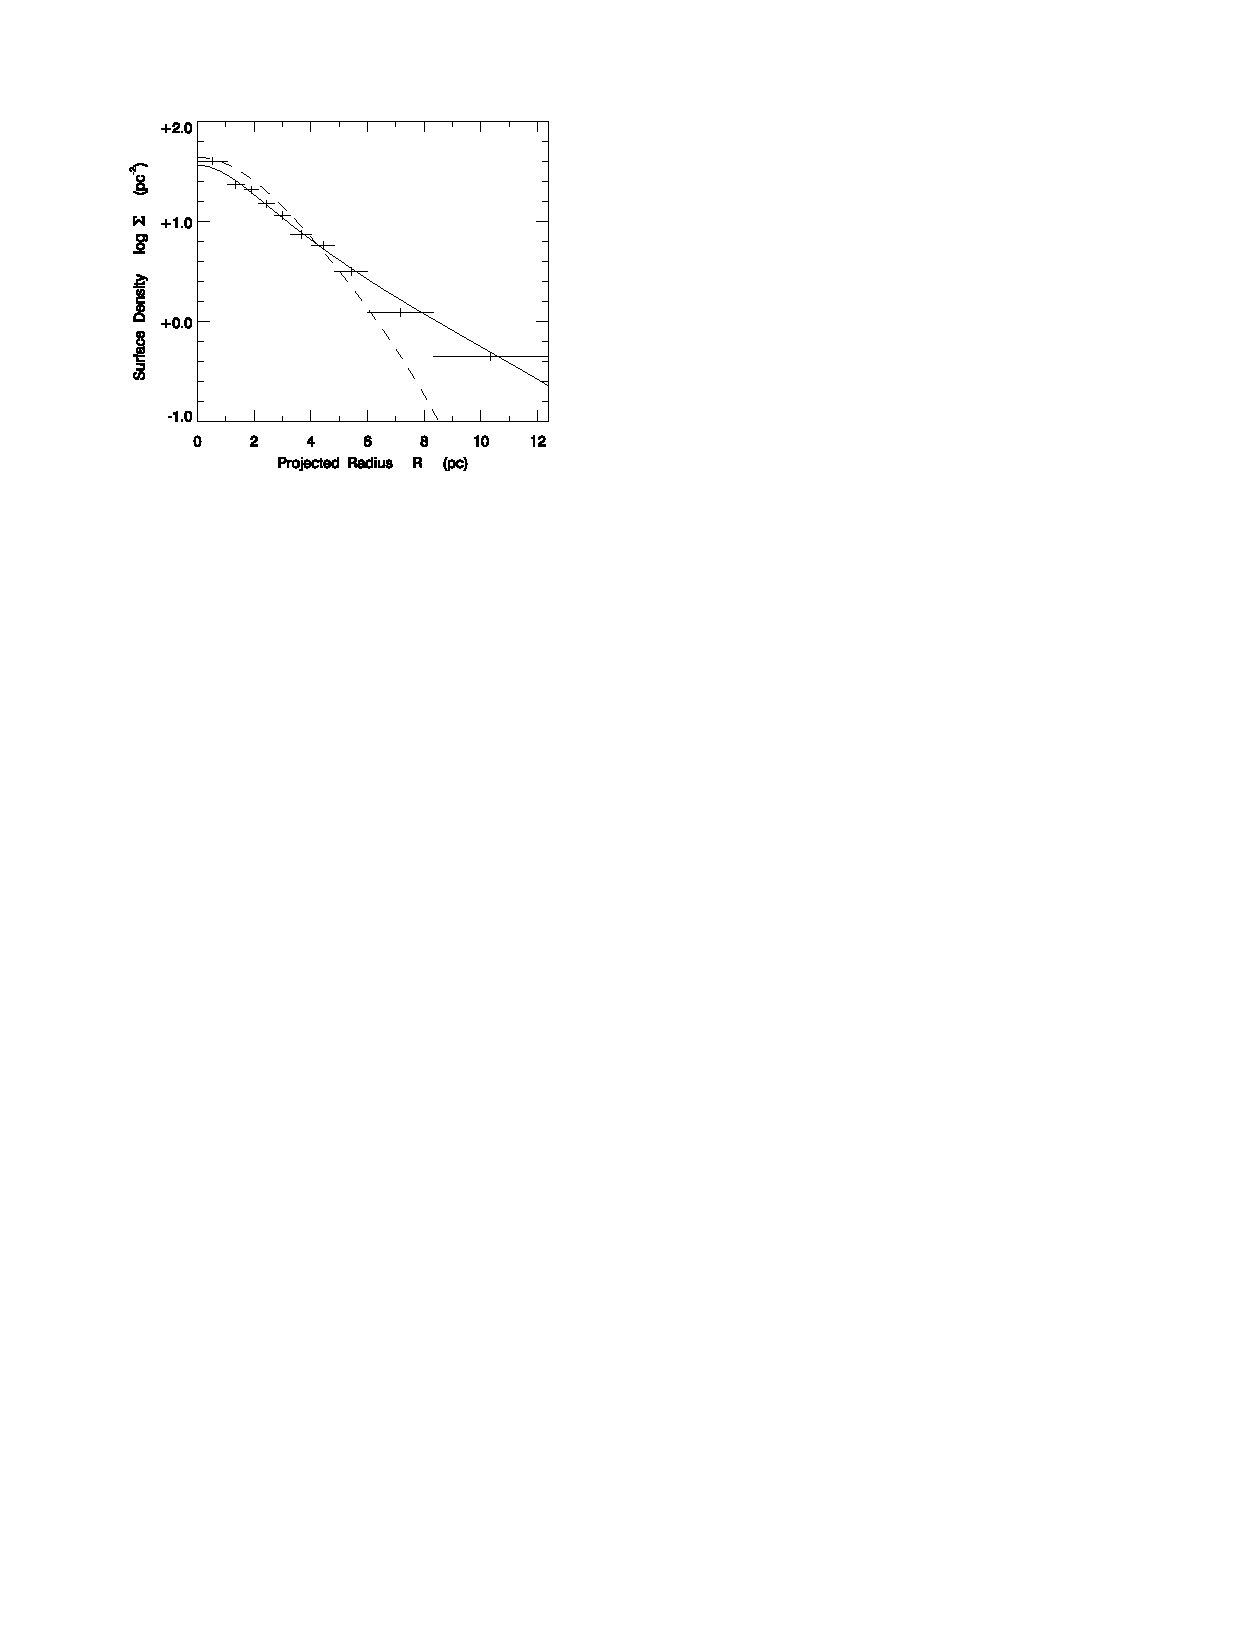
\includegraphics[height=6cm]{background/Figures/F1_Converse2010.pdf}
        \caption{}
        \label{fig:spatialConverse}
    \end{subfigure}
    \begin{subfigure}[t]{0.49\textwidth} \centering
       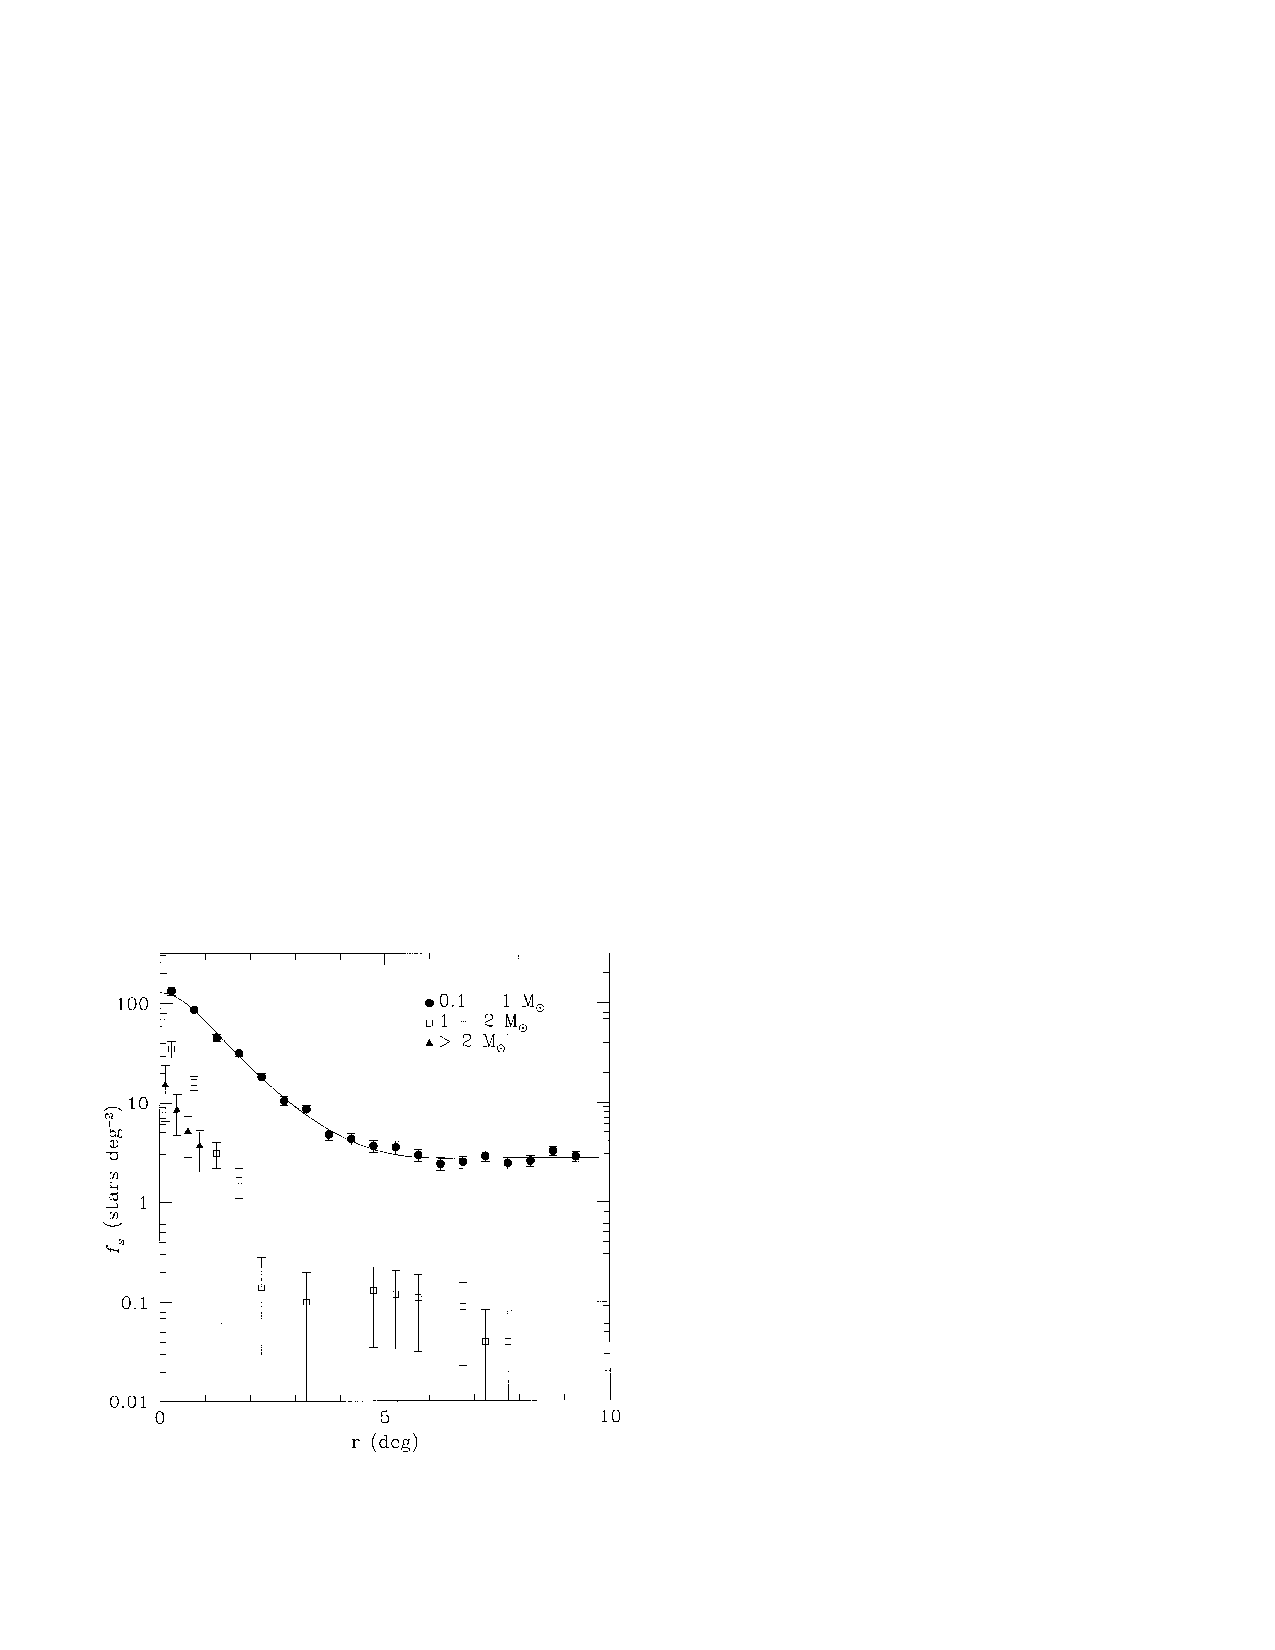
\includegraphics[height=6cm]{background/Figures/F8_Adams2001.pdf}
        \caption{}
        \label{fig:spatialAdams} 
    \end{subfigure}
    \caption{Projected spatial distribution of the Pleiades cluster. (a) Results from  \citet{Converse2010}. The crosses, and the dashed and solid lines represent the data and the fitted polytrope and King profile, respectively. Reproduced from Figure 1 of \citet{Converse2010}, \textit{\usebibentry{Converse2010}{Title}}, \usebibentry{Converse2010}{Journal}, Vol. \usebibentry{Converse2010}{Volume}. (b) Results from \citet{Adams2001}. The line shows the fitted King profile while the symbols are for different mass bins used. Reproduced from Figure 8 of \citet{Adams2001}, \textit{\usebibentry{Adams2001}{Title}}, \usebibentry{Adams2001}{Journal}, Vol. \usebibentry{Adams2001}{Volume}.}
\end{figure}

\begin{table}[ht!]
\caption{Survey, and derived core and tidal radius for recent studies in the literature. }
\begin{center}
\begin{tabular}{ccccc}
Authors &Core&Tidal& Tidal & Survey\\
&radius&radius&radius&radius\\
&(pc)&(pc)&($^\circ$)&($^\circ$)\\
\hline
\citet{Pinfield1998}&0.9-2.91&13.1&5.6&3\\
\citet{Raboud1998}&1.5&17.5&7.5&5\\
\citet{Adams2001}&2.35-3.0&16&6.8&10\\
\citet{Converse2008}&1.3&18&7.7&5\\
\citet{Converse2010}&2.0&19.5&8.3&5\\
\hline
\end{tabular}
\end{center}
\label{tab:tidal_iterature}
\end{table}%

  
\section{Velocity Distribution}

The three dimensional velocity distribution of the Pleiades has also been studied using its projections. One of them goes along the line of sight, it corresponds to the radial velocity. The other one is perpendicular to the previous one, lies in the plane of the sky, and corresponds to the transverse velocity. It is derived from  proper motions. These are angular velocities obtained after measuring the angular displacement of the object in at least two different epochs. Again, measuring the individual stellar position and its displacement over time is far easier than measuring radial velocities. These are measured using the Doppler shifted absorption lines in the spectre of the object. This shift is proportional to the object velocity relative to the observer along the line of sight. 

Since radial velocities require the object spectrum, their obtention for all cluster members, and particularly for the fainter ones, will demand a large amount of observing time. On the other hand, wide field images have been available for quite a long time, thus allowing long time base lines to measure proper motions.  Nevertheless, due to the Pleiades distance, radial velocities are often more precise than proper motion measurements, usually on the $1 \,\mathrm{km\cdot s^{-1}}$ regime. For these reasons, historically, the velocity distribution of the Pleiades cluster has been studied through the proper motions of its members. 

Probably the first description of the \gls{tvd} of the Pleiades is that of \citet{1884MNRAS..44..355P}. Using archival data from  Königsberg (1838-1841), Paris(1874) and Oxford (1878-1880) observatories, together with his own \emph{Differential Micrometer} observations, he was able to observe the relative displacements of 40 Pleiades stars. According to him \citep{1884MNRAS..44..355P}: \textit{the relative displacements of these distant suns, although not distinctly and accurately measurable in numerical extent, appear to vary both in direction and amount; indicating thereby the mutual influence of a group of gravitating bodies.} 

Later, \citet{Trumpler1921} used, for the first time, proper motion measurements to identify the members of the Pleiades cluster. He classified objects as candidate members according to the distance they show, in the proper motion space, to the mean proper motion of the cluster. This mean was previously calculated by Boss in his \emph{Preliminary General Catalog} \citep{1910pgcs.book.....B}. So far as my historic research went, Boss' work was the first measurement of a statistic of the \gls{tvd} of the Pleiades. 

Later \citet{1938AJ.....47...25T}, using Trumpler's data and archival compilations, was able to measure the dispersion of the proper motions distribution. He estimated it to be $0.79\,\mathrm{mas\cdot yr^{-1}}$($0.65\,\mathrm{ km\cdot s^{-1}}$ at 136 pc). This was probably, the first measurement of the second moment of the spatial velocity distribution. From this value he then derived a total mass of $260\,\mathrm{M_{\odot}}$.

In recent years \citet{Pinfield1998} used the velocity dispersion to probe that the cluster was in an state near to the virial equilibrium. Later, \citet{2006ARep...50..714L} used the projected radial and tangential velocity components of the spatial velocity distribution of 340 members to claim the absence of evidence for rotation, expansion or compression of the cluster. Also, he also found no evidence to support mass segregation. 

Concerning the radial velocities, the first record for the Pleiades correspond to \citet{1904ApJ....19..338A}. He measured the radial velocities of the six brightest stars. After this seminal work, more than a dozen of works have been published. Among them are the works of \citet{1924PhDT.........1W,1944ApJ...100..360S,1979BICDS..16....2M,1991ApJ...377..141L,1992A&A...255..130R,1994AJ....108..160S,1997A&A...320...74M,1996ApJ...469..706M,2000AJ....119.1303T,2006ARep...50..714L,2009AAS...21340702W,2009A&A...498..949M}, and \citet{2013AJ....146..134K}. In previous studies, the typical number of Pleiades candidate members was below 100 objects, with the works of \citet{2009AAS...21340702W} and \citet{2009A&A...498..949M} reaching 269 and 275 objects, respectively. The latest compilation of radial velocities from the literature is the one made made by \citet{Galli2017}. This list contains measurements for 394 objects. The distribution of these radial velocities is almost gaussian with a centre at $5.6\,\mathrm{km \cdot s^{-1}}$. In \citet{Galli2017}, we estimated a velocity dispersion of the $0.8\,\mathrm{ km\cdot s^{-1}}$ for the Pleiades candidate members.

Although, transverse and radial velocities are useful projections, the dynamical analysis of the cluster demands the three dimensional distribution. In \citet{Galli2017} we provide a list of 64 cluster members with full spatial velocities. The distributions of the three projections of these spatial velocities are shown in Figure \ref{fig:velocityGalli}.

\begin{figure}[ht!]
\begin{center}
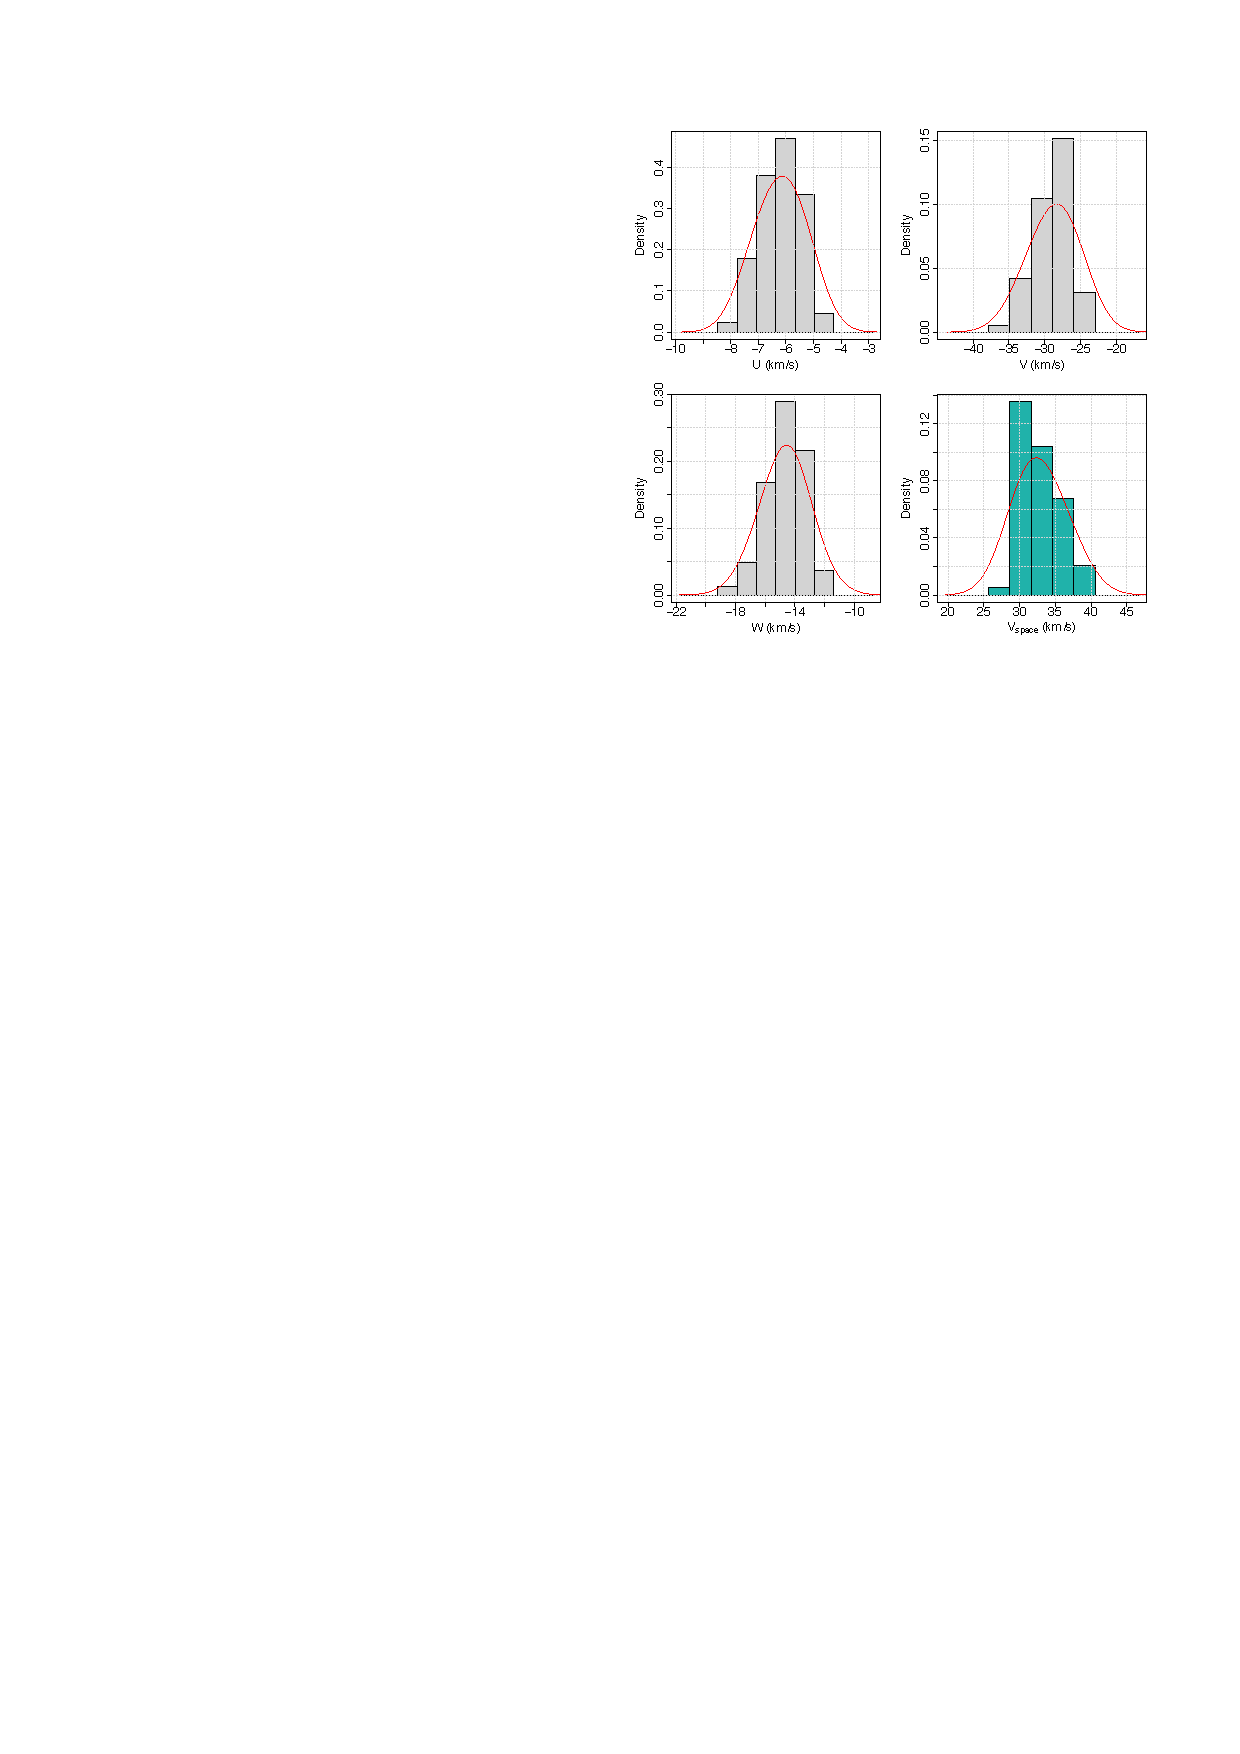
\includegraphics[width=0.8\textwidth]{background/Figures/F11_Galli2017.pdf}
\caption{Histogram and kernel density estimation (red line) of the components (grey) and modulus (green) of the spatial velocity distribution of 64 candidate members of \citet{Galli2017} with radial velocities and parallaxes. Reproduced from Figure 11 of \citet{Galli2017}, \textit{\usebibentry{Galli2017}{Title}}, \usebibentry{Galli2017}{Journal}, Vol. \usebibentry{Galli2017}{Volume}.}
\label{fig:velocityGalli}
\end{center}
\end{figure}

\section{Luminosity Distribution}

The luminosity distribution usually refers to the statistical probability distribution of the absolute\footnote{The absolute magnitude $M$, is the brightness that an object of apparent magnitude $m$ will show at a distance of 10 pc.} magnitude of the cluster population. It can also refer to the distribution of apparent magnitudes. It can be thought as the spectrum of brightness of the cluster members. Its importance lies in the fact the the luminosity of a star, measured in absolute magnitudes, can be related to its mass by the mass-luminosity relation. Therefore, the luminosity distribution is a proxy for the mass distribution. 

The study of the distribution of luminosities in the Pleiades started few years later than those of the positions and proper motions. The first record I found on the luminosity distribution is the one of \citet{Trumpler1921} (see Fig. \ref{fig:luminosityTrumpler}). He computed the number of stars in each magnitude bin for his two samples of candidate members, those comprising the objects within the central $1^{\circ}$, and those between $1^{\circ}$ and $3^{\circ}$, referred as Tables I and II, respectively. The completeness of the inner and outer samples was estimated at 14.5 and  9.8 photographic magnitudes (roughly 14 and 9 in the visual band), respectively. He observed that the luminosity distributions of these two samples were not alike, with the inner sample being brighter than the outer one. He also noticed that the luminosity distribution is not smooth, and shows a local minimum at 9 magnitudes, then an abrupt rise. Both effects are present in the two samples.

\begin{figure}[ht!]
\begin{center}
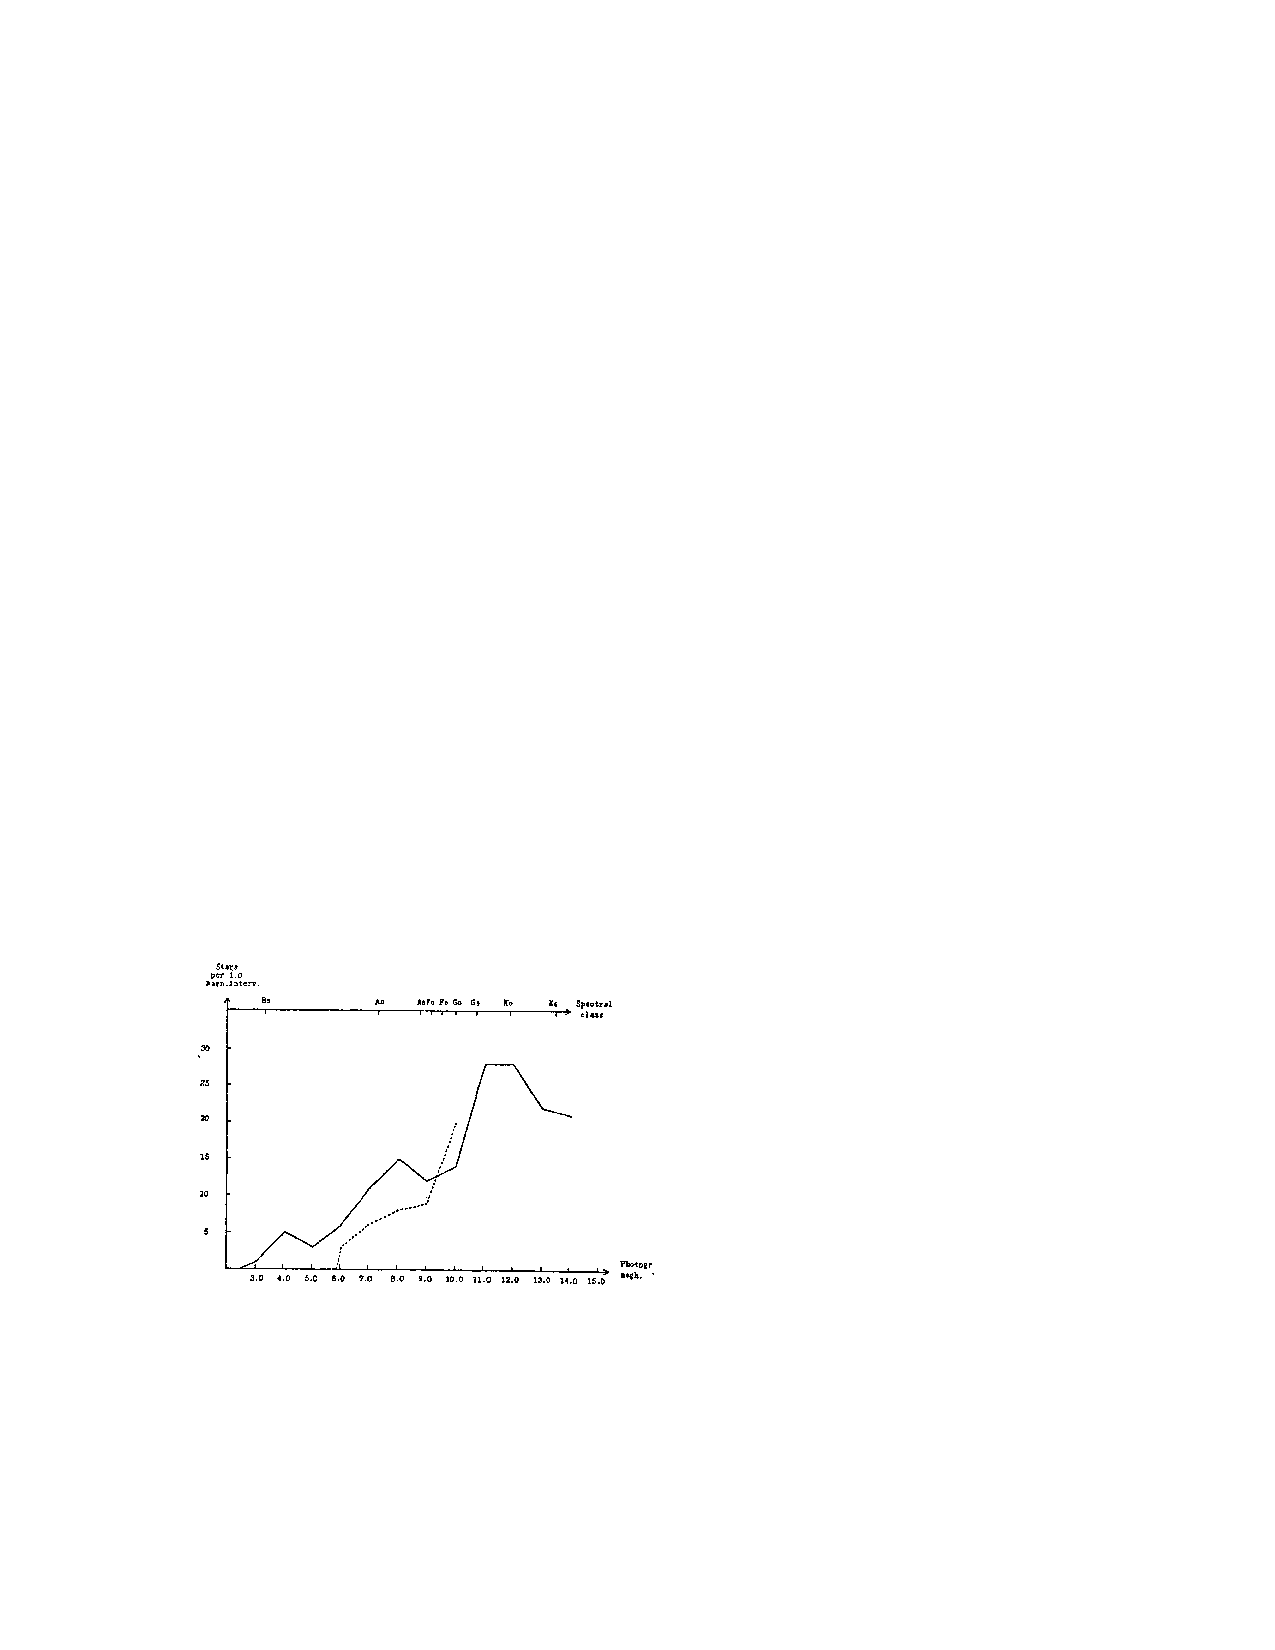
\includegraphics[width=\textwidth]{background/Figures/F2_Trumpler1921.pdf}
\caption{Luminosity distribution according to \citet{Trumpler1921}. The solid and dashed lines correspond to objects within $1^{\circ}$ and within $1^{\circ}$, and $3^{\circ}$ from the centre. Reproduced from Figure 2 of \citet{Trumpler1921}, \textit{\usebibentry{Trumpler1921}{Title}}, \usebibentry{Trumpler1921}{Journal}, Vol. \usebibentry{Trumpler1921}{Volume}.}
\label{fig:luminosityTrumpler}
\end{center}
\end{figure}

Later, \citet{Johnson1958} obtained the luminosity distribution using a sample of 289 candidate members. They assessed  membership solely on photometry. Their luminosity distribution is shown in Fig. \ref{fig:luminosityJohnson}

\begin{figure}[ht!]
\begin{center}
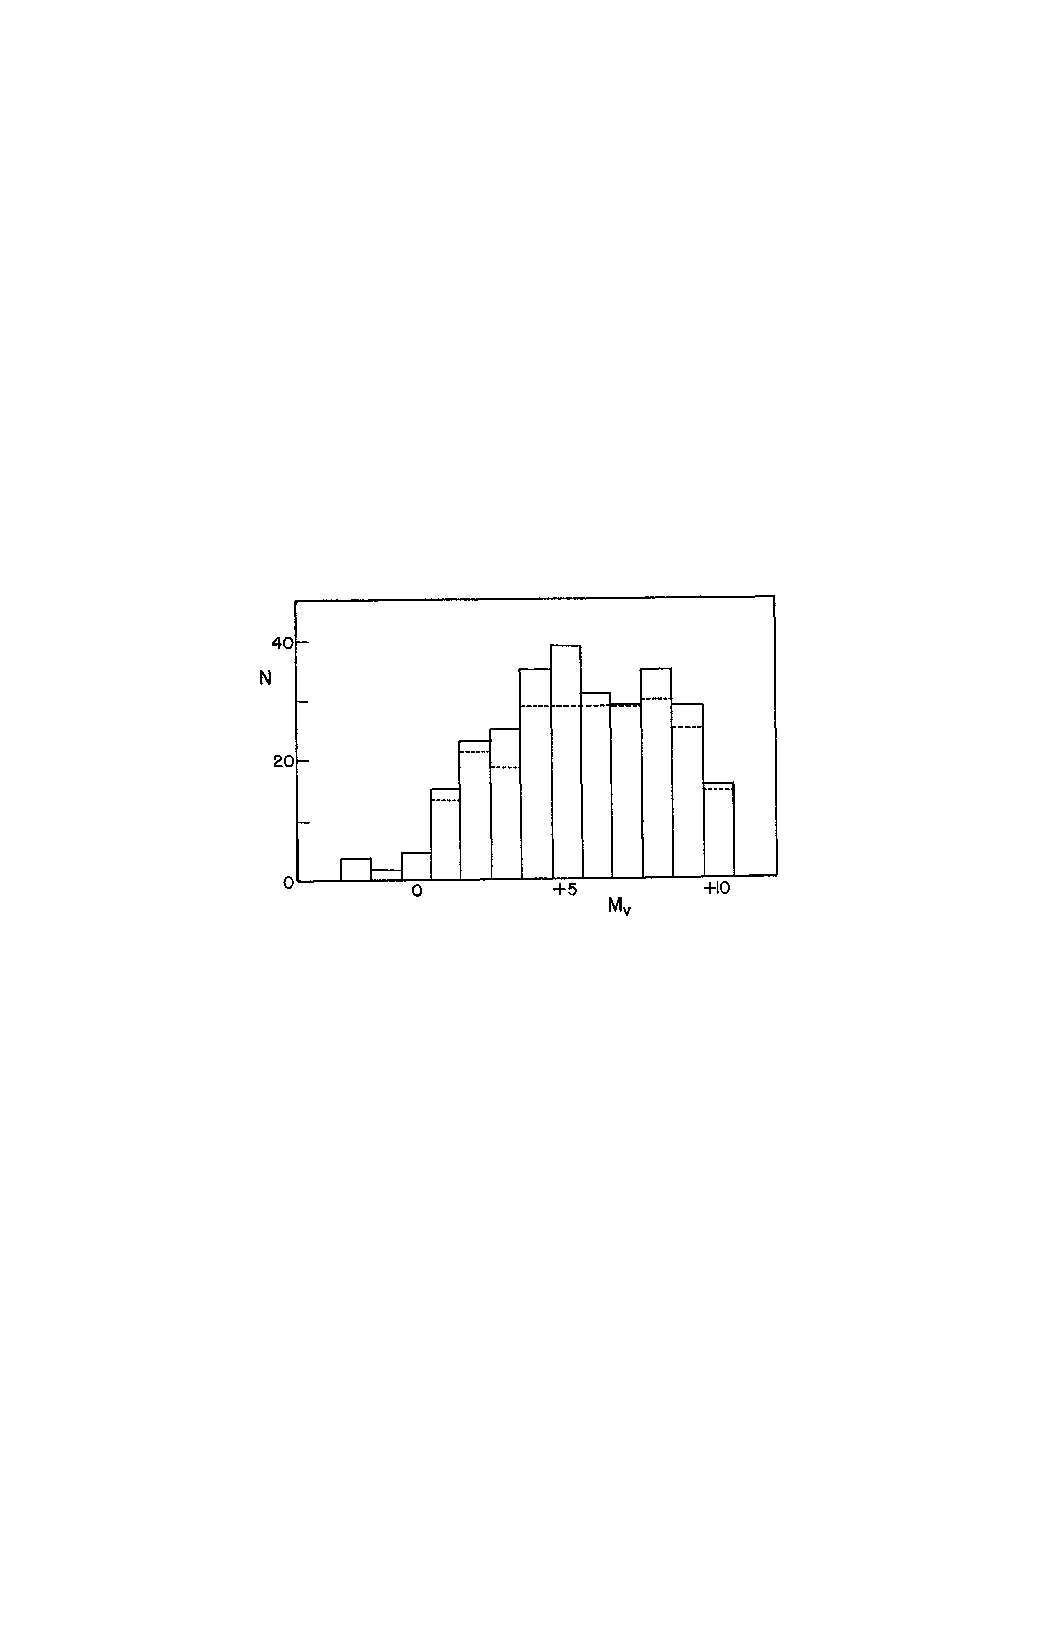
\includegraphics[height=8cm]{background/Figures/F3_Johnson1958.pdf}
\caption{Luminosity distribution in the visual band according to \citet{Johnson1958}. The dotted line represent the counts of main sequence stars only. Reproduced from Figure 3 of \citet{Johnson1958}, \textit{\usebibentry{Johnson1958}{Title}}, \usebibentry{Johnson1958}{Journal}, Vol. \usebibentry{Johnson1958}{Volume}.}
\label{fig:luminosityJohnson}
\end{center}
\end{figure}

Later, \citet{Limber1962} compared the luminosity distributions derived from the data of \citet{Trumpler1921}, \citet{Hertzsprung1947}, and \citet{Johnson1958}, with the initial luminosity distribution that he derived \citep{Limber1960}. The initial luminosity distribution corresponds to the distribution of luminosities that the cluster had at the moment of formation. \citet{Limber1960} derived it mixing data of galactic clusters and the local neighbourhood, and later correcting it by effects of age. He noted that the Pleiades present day luminosity distribution starts to differ from the initial luminosity distribution at visual magnitude $5.5$, see Fig. \ref{fig:luminosityLimber}. Assuming that this difference is due to the fact that stars fainter than $5.5$ have not yet had enough time for contraction, he derives an age of 50 \gls{myr}. 

\begin{figure}[ht!]
\begin{center}
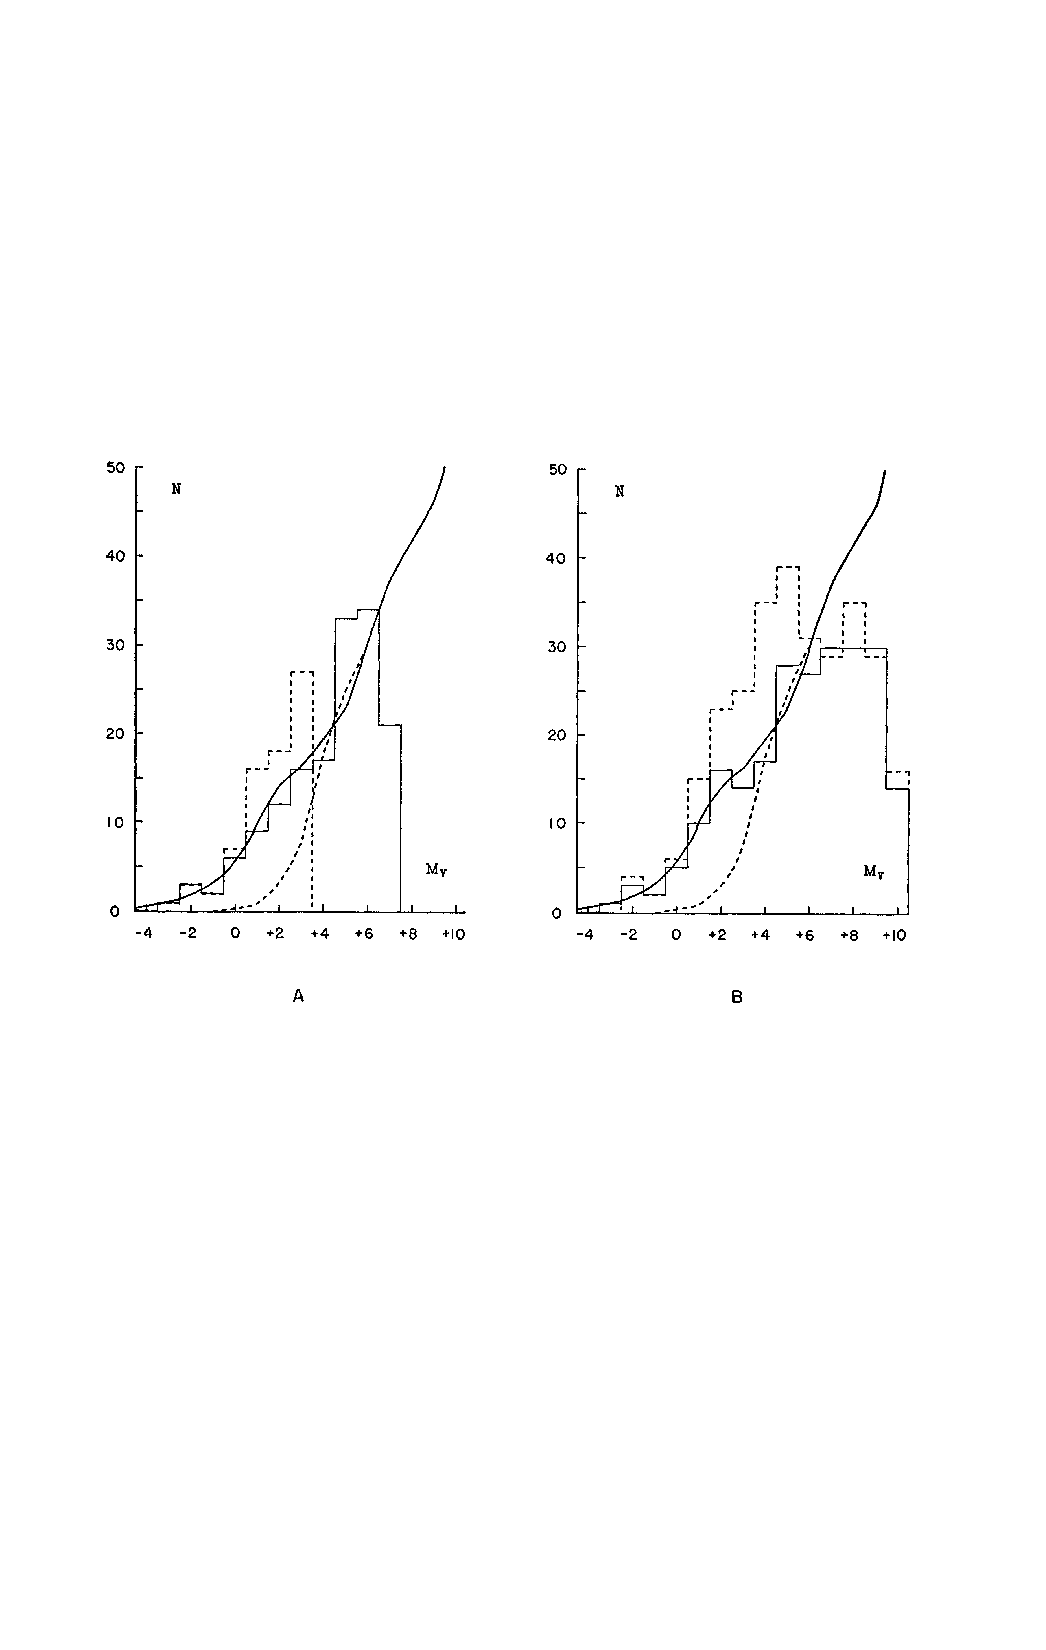
\includegraphics[height=8cm]{background/Figures/F4_Limber1962.pdf}
\caption{Luminosity distribution in the visual band according to \citet{Limber1962}.The solid and dashed histograms in: A correspond to \citet{Trumpler1921} data from the Tables II and I, respectively, in B, correspond to the data from \citet{Hertzsprung1947} and \citet{Johnson1958}, respectively. The solid and dashed curves line represent initial luminosity distribution and the present day luminosity distribution of the solar neighbourhood, respectively, both from \citet{Limber1960} . Reproduced from Figure 4 of \citet{Limber1962}, \textit{\usebibentry{Limber1962}{Title}}, \usebibentry{Limber1962}{Journal}, Vol. \usebibentry{Limber1962}{Volume}.}
\label{fig:luminosityLimber}
\end{center}
\end{figure}

In recent years, the luminosity distribution has been described in the works of \citet{Lodieu2012} and \citet{Bouy2015}. 
\citet{Lodieu2012}, using the \emph{UKIDSS} DR9 survey for galactic clusters and a probabilistic membership selection method (see discussion in Chapter \ref{chap:introduction}) based on proper motions only, and proper motions and photometry, found 8797 and 1147 candidate members, respectively. However, they do not provide the contamination rate in their analysis. Using both lists, they provide their luminosity distributions in the $Z$ band, which I show in Fig. \ref{fig:luminosityLodieu}.

\begin{figure}[ht!]
\begin{center}
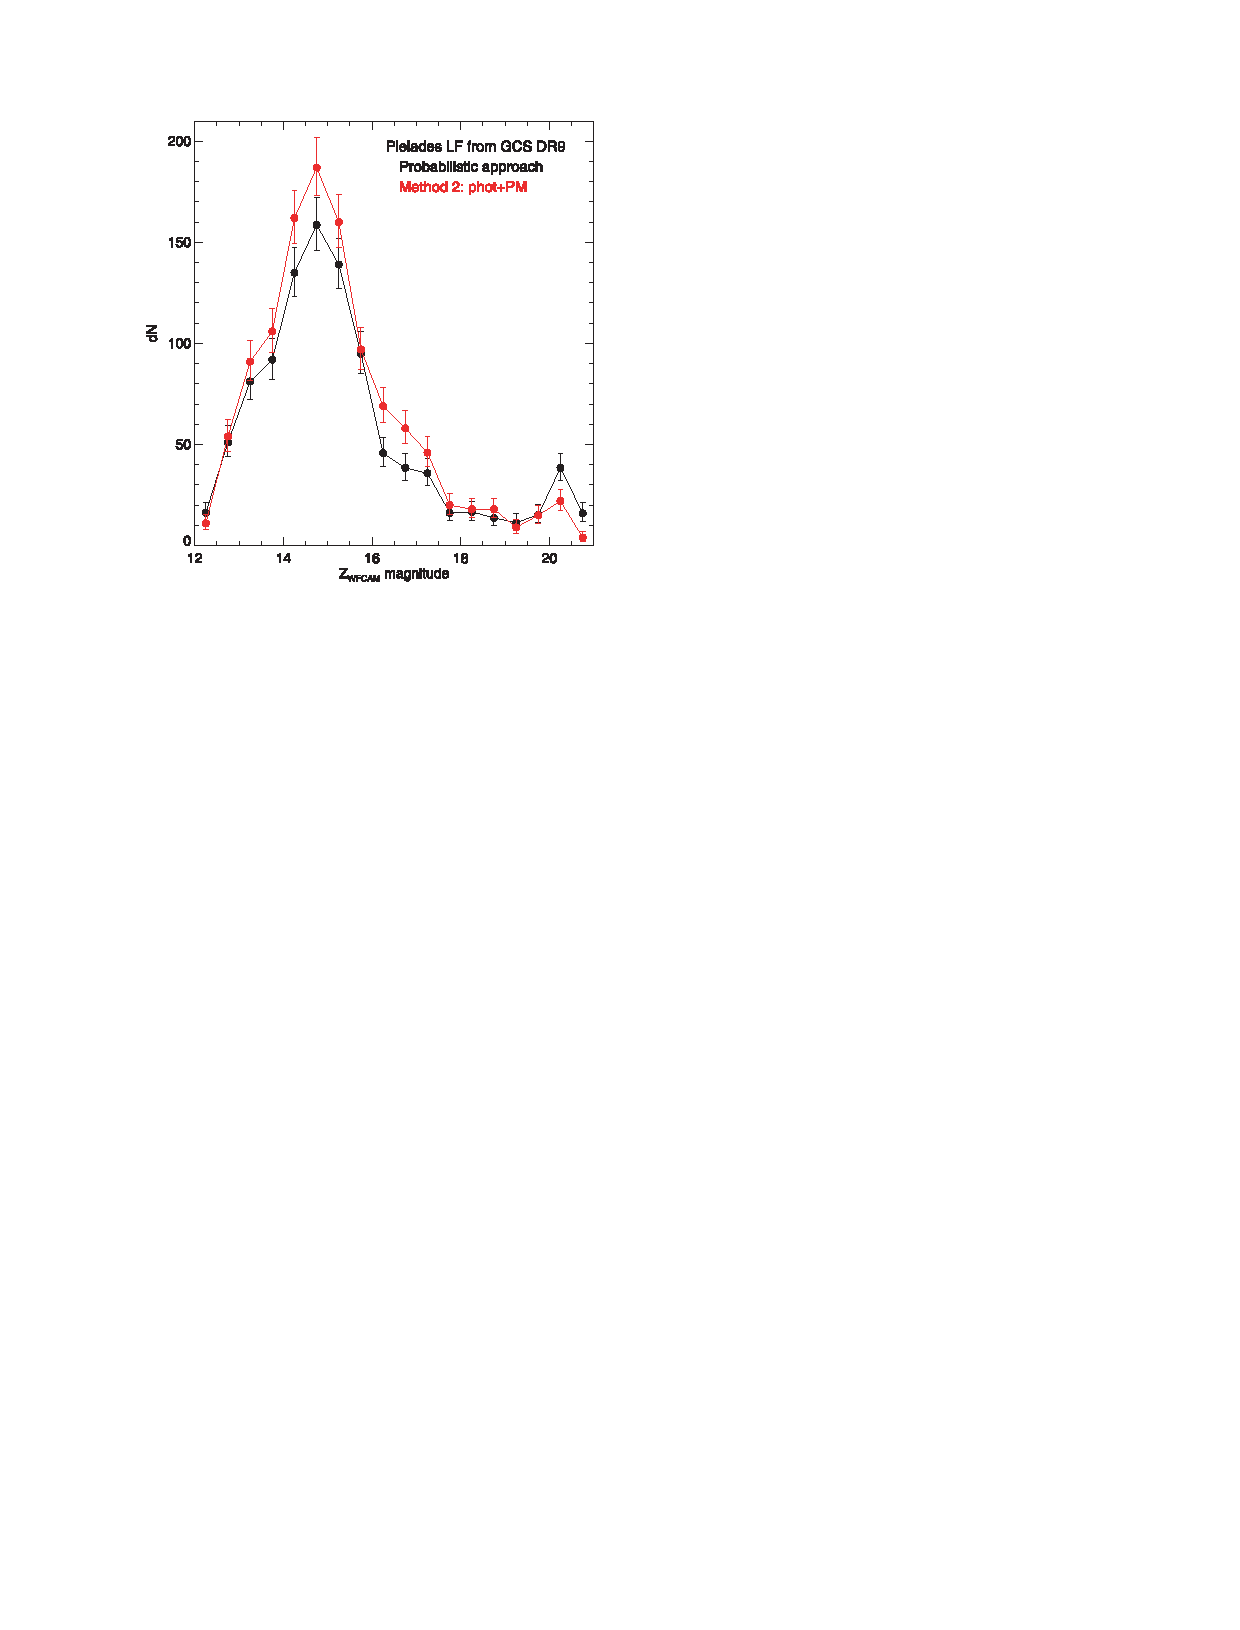
\includegraphics[height=8cm]{background/Figures/F9_Lodieu2012.pdf}
\caption{Luminosity distribution  in the $Z$ band according to \citet{Lodieu2012}. The red and black lines correspond to the two different probabilistic methods.  Reproduced from Figure 9 of \citet{Lodieu2012},\textit{\usebibentry{Lodieu2012}{Title}}, \usebibentry{Lodieu2012}{Journal}, Vol. \usebibentry{Lodieu2012}{Volume}.}
\label{fig:luminosityLodieu}
\end{center}
\end{figure}

In \citet{Bouy2015},  we estimated the present day system luminosity distribution of 1378 candidate members contained within the central $3^{\circ}$ region (with the centre at R.A.$=03:46:48$ and Dec.$=24:10:17$ J2000.0). It is called systemic because it has not been corrected for unresolved systems. An unresolved system is a group of stars (e.g. binaries) that due to its compactness appears as a single object. This distribution was computed for the $K_s$ band and is sensitive up to $K_s \sim 20$ mag and complete until $K_s \sim 17$ mag. This luminosity distribution is reproduced in Fig. \ref{fig:luminosityBouy}


\begin{figure}[ht!]
\begin{center}
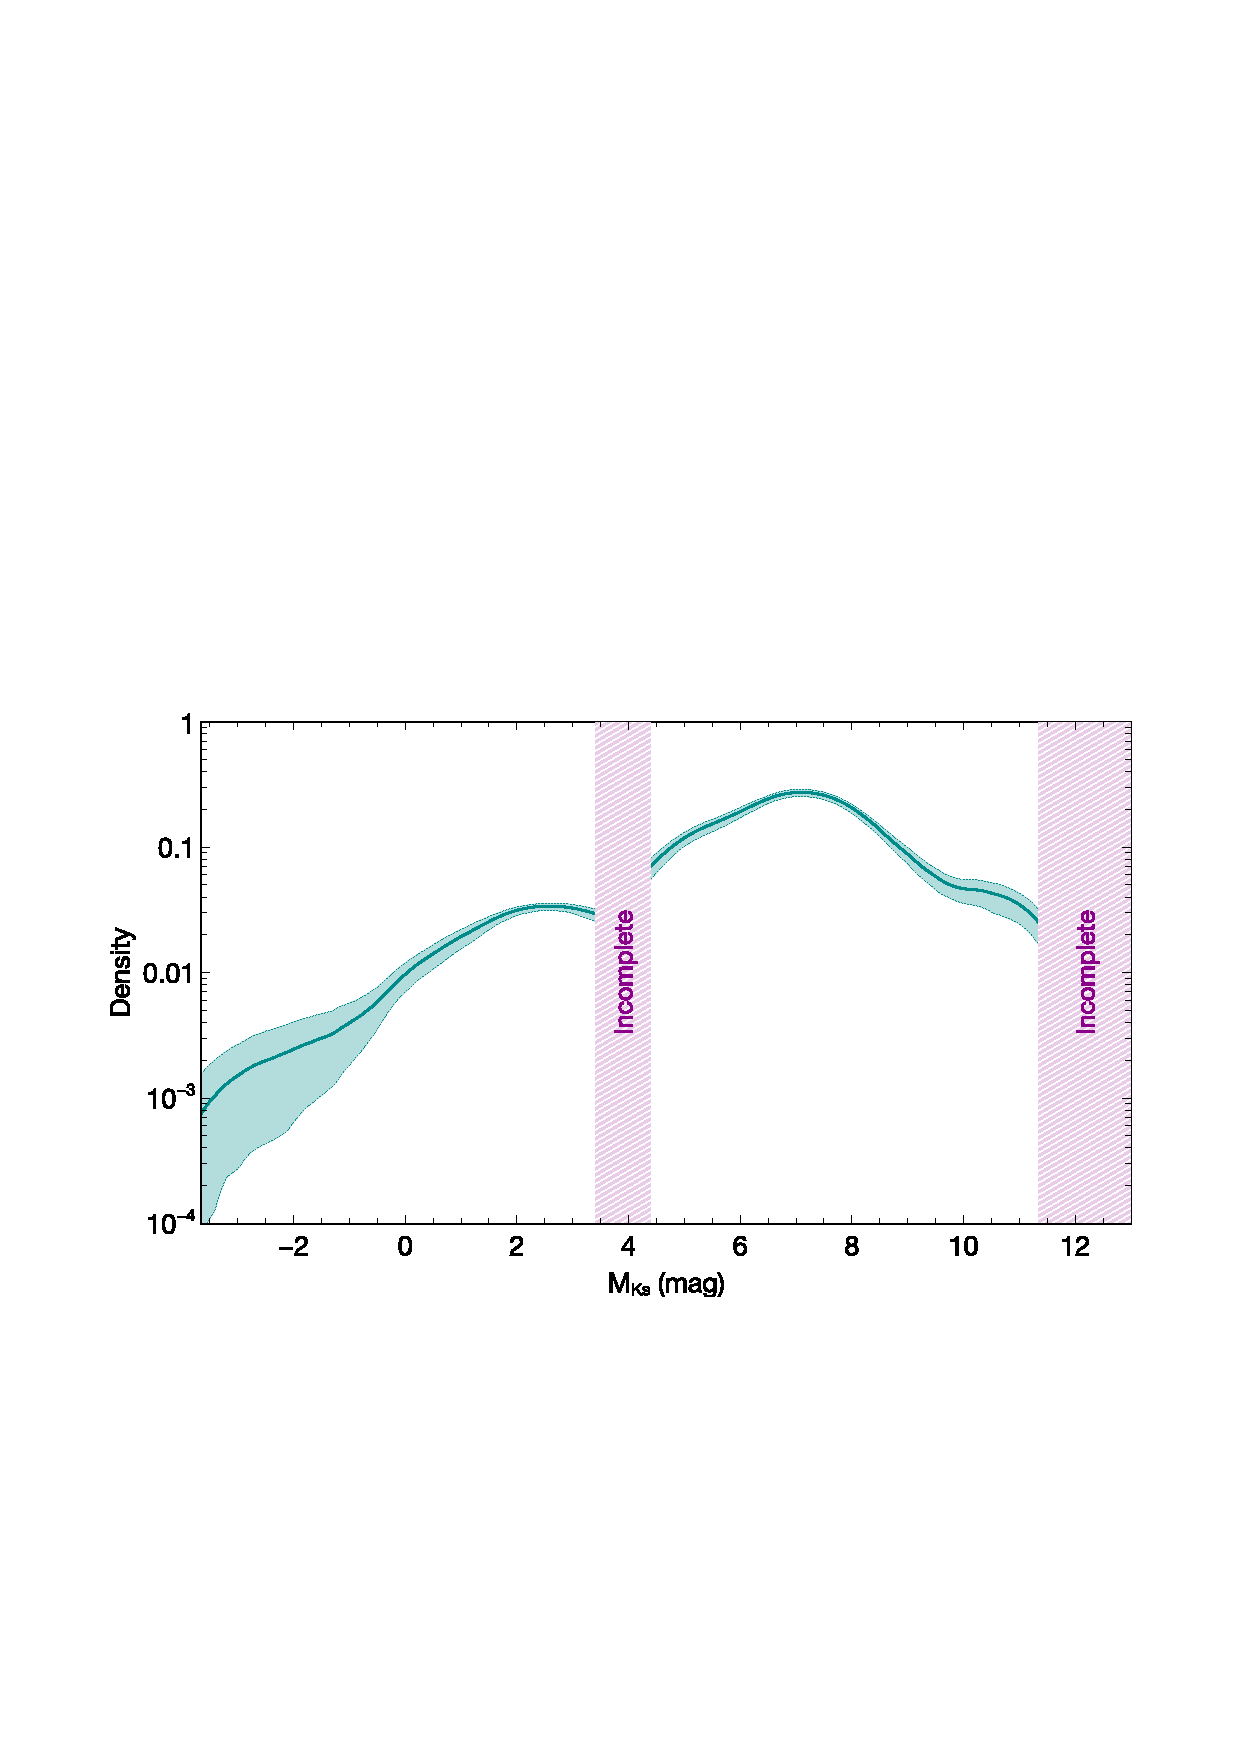
\includegraphics[width=\textwidth]{background/Figures/F8_Bouy2015.pdf}
\caption{Luminosity distribution in the $K_s$ band according to \citet{Bouy2015}. The incompleteness regions are shaded. Reproduced from Figure 8 of \citet{Bouy2015},\textit{\usebibentry{Bouy2015}{Title}}, \usebibentry{Bouy2015}{Journal}, Vol. \usebibentry{Bouy2015}{Volume}.}
\label{fig:luminosityBouy}
\end{center}
\end{figure}

\section{Mass Distribution}
\label{sect:mass}

In astrophysics, the mass distribution is a cornerstone in the understanding of the star formation process and the later evolution of stellar systems. Although the temporal evolution of these systems is mainly dominated by the gravitational potential, the initial conditions and an ongoing star formation process, if any, can contribute to the shape of the mass distribution. This last contains the fingerprints of past events in the history of the cluster and plays a key roll in its future evolution. Indeed, the evolution of the mass distribution is an essential element in one of modern astrophysics' objectives: the determination of the roll played by the initial conditions or the environment, in the temporal evolution of the stellar systems. The mass distribution at the moment of the cluster formation, which is known as the initial mass distribution evolves in time according to: i) stellar internal and atmospheric processes (e.g. contraction, mass loss, inflation, supernova events), ii) population dynamical interactions (e.g. three-body encounters, runaway stars, stellar evaporation), and iii) galactic dynamics (e.g. tidal effects, encounters with other clusters). For these reasons, the study of the initial mass function and its posterior evolution is a key element in the current understanding not just of open clusters but also of galactic and extragalactic populations.  


The mass distribution of the Pleiades has been largely studied. The first work on the mass distribution is that of \citet{Limber1962}. Although he did not show any graphical or tabular representation of it, he gave the luminosity distribution and the mass-luminosity ratio. Form these the mass distributions can be derived. Instead, he use them to obtain the total mass of the cluster ($760\,\mathrm{M_{\odot}}$, see next Section). 

Most probably, the first work to present the mass distribution derived from luminosity distributions and a mass-luminosity relation from theoretical models was that of \citet{Hambly1991}. Using $R$ and $I$ observations from the \emph{United Kingdom Schmidt Telescope Unit} together with the mass-luminosity relation from theoretical isochrone models of Padova group, he was able to transform his luminosity distribution into a mass distribution. In Fig. \ref{fig:massHambly}, I reproduce his results. 

\begin{figure}[ht!]
\begin{center}
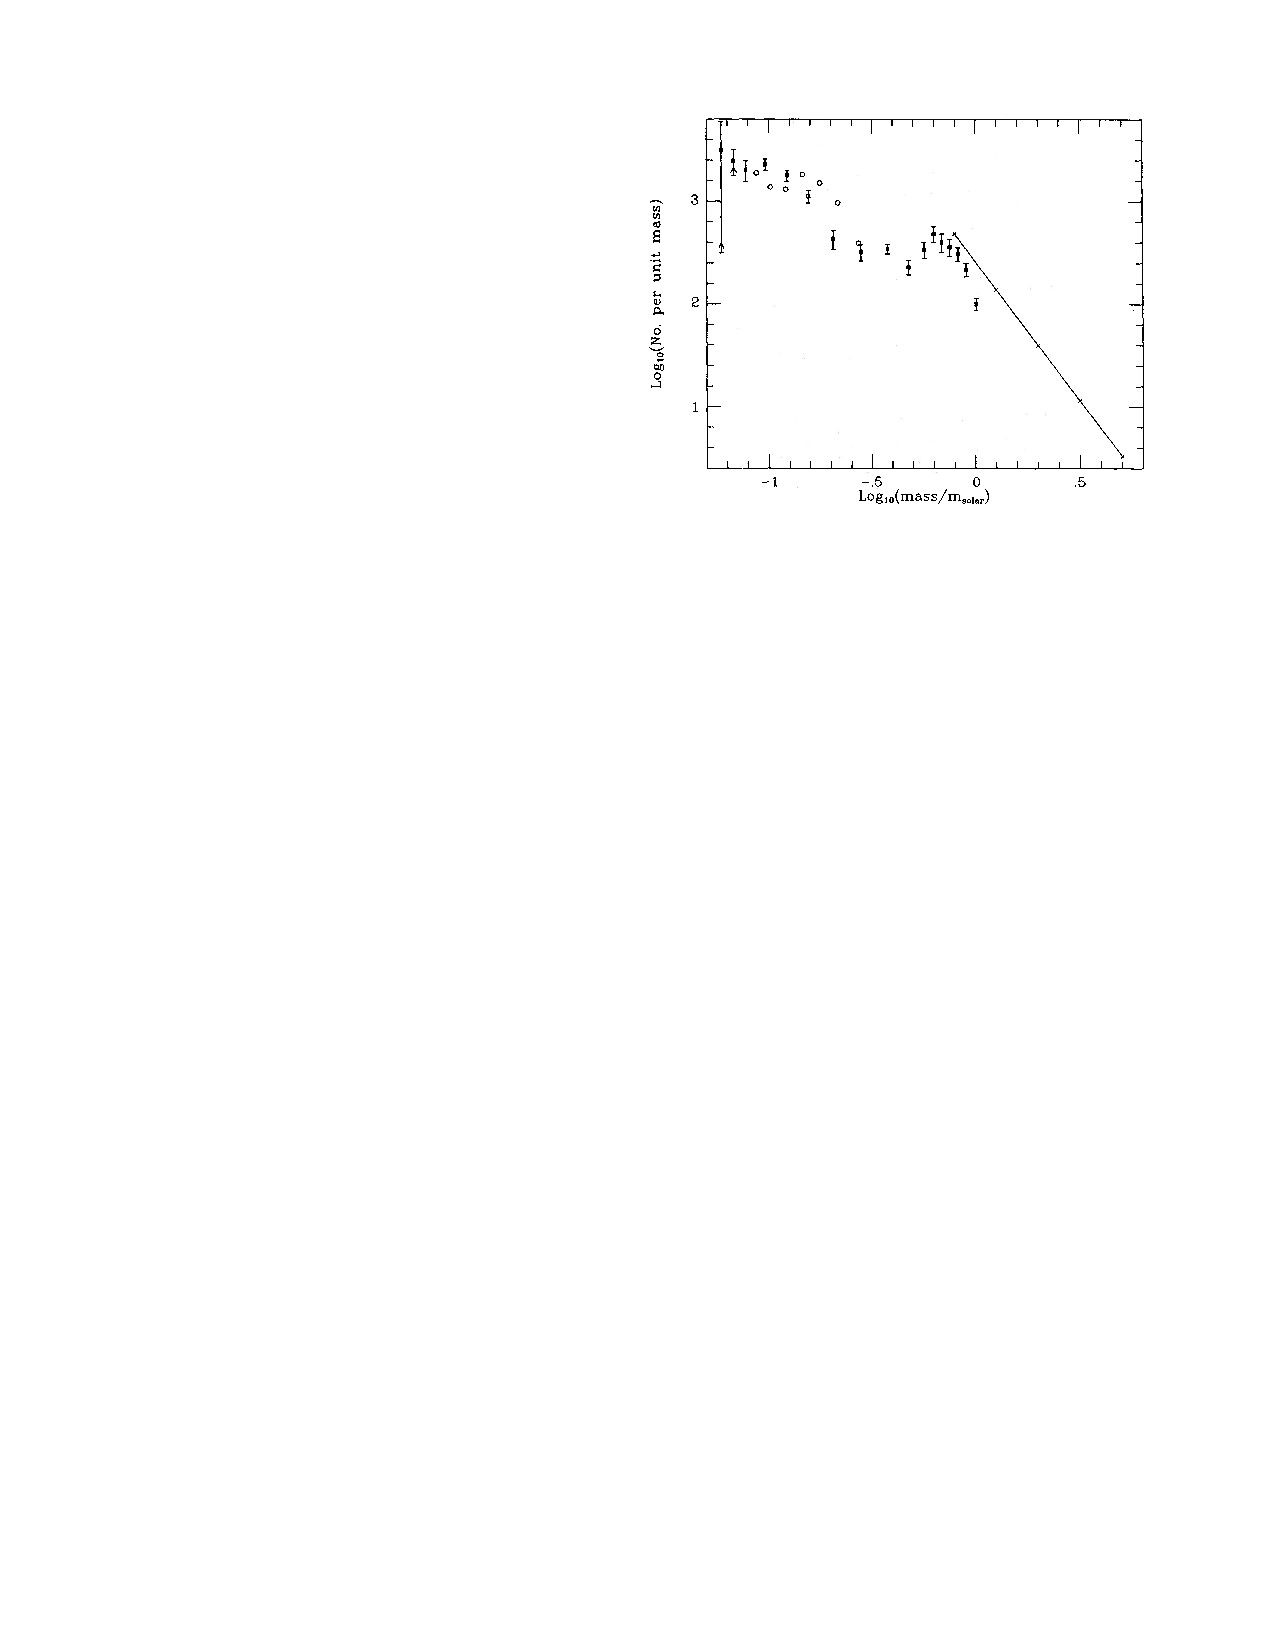
\includegraphics[height=8cm]{background/Figures/F11_Hambly1991.pdf}
\caption{Mass distribution of \citet{Hambly1991} derived from luminosity distribution and theoretical isochrone models. The open circles result from assuming an older age of 200 \gls{myr}. The line represent the mass distribution of \citet{1980IAUS...85..157V}. Reproduced from Figure 11 of \citet{Hambly1991},\textit{\usebibentry{Hambly1991}{Title}}, \usebibentry{Hambly1991}{Journal}, Vol. \usebibentry{Hambly1991}{Volume}.}
\label{fig:massHambly}
\end{center}
\end{figure}

From the year 2000 till date, several studies have been published in which the subject of analysis is the Pleiades mass distribution, e.g. \citet{2000ASPC..198...59H, 2002MNRAS.335..853J, 2001A&A...367..211M,2003A&A...400..891M, 2004A&A...426...75M, 2007MNRAS.380..712L}. However, for the sake of simplicity, here I only analyse the two most recent works, those of \citet{Lodieu2012} and \citet{Bouy2015}. The \gls{pdsmd} derived from both these works are shown in Figs. \ref{fig:massLodieu} and \ref{fig:massBouy}. These works obtained first the luminosity distribution, and then transformed it into a mass distributions using mass-luminosity relations of theoretical isochrone models. 

\citet{Lodieu2012} used a distance of 120.2 pc, an age of 120 \gls{myr}, and the \emph{NEXTGEN} theoretical models of \citet{1998A&A...337..403B} to transform the luminosity into the mass distribution. On the other hand, in \citet{Bouy2015} we use a distance of 136.2 pc an age of 120 \gls{myr} and the \emph{BT-Settl} theoretical isochrone models of \citet{2014IAUS..299..271A}. 

Both works found that their derived \gls{pdsmd} are in general agreement with the \gls{imf} of \citet{Chabrier2005} for unresolved systems (see Section \ref{sect:IMF}). However, in \citet{Bouy2015} we pointed out that, assuming that the theoretical mass-luminosity relation is correct, the \glspl{imf} of \citet{Chabrier2005} and \citet{Thies2007} predict too many low-mass stars and brown dwarfs in the range $0.04-0.1\,\mathrm{M_{\odot}}$. 

The differences at the low mass regime between the \gls{pdsmd} derived by \citet{Lodieu2012} and \citet{Bouy2015} (see Figs. \ref{fig:massLodieu} and \ref{fig:massBouy}) could arise from the different i) samples of members, ii) mass-luminosity relations, and iii) distances adopted by both works.

The different distances can introduce a general shift in the luminosity, which in turn can shift the mass distribution. This shift in luminosity, however, can be neglected due to its small value, $0.06$ mag.

Concerning the differences between the mass-luminosity relations of the two isochrone models, \citet{2013MmSAI..84.1053A} show that there are clear differences between the effective temperatures delivered by the \emph{BT-Settl} and the \emph{NEXTGEN} models in the low-mass regime, at $5$ Gyr particularly. {However, they do not discuss how this difference change in younger ages. Thus, this effect can not be discarded as the source of the differences.}

Concerning the differences between the lists of candidate members, \citet{Lodieu2012} do not provide (at least explicitly) any estimate of contamination rate of their samples. Furthermore, their membership methodology has some draw backs \cite[see][]{Sarro2014} that may have biased their results. {Therefore, the agreement that \citet{Lodieu2012} found between their present day mass distribution and the \gls{imf} of \citet{Chabrier2005}, which models the field mass distribution, may be an indication that their sample of candidate members is contaminated by the field.  }

On the other hand, in \citet{Bouy2015} we estimated a contamination rate of 7\%. However, we have no evidence for it to be non-homogeneous in mass. Even if the 7\% contaminants were not homogeneously distributed in the mass range, this value is not able to account for the observed discrepancies ($30-40\%$ in the low-mass regime) between the \gls{imf} of \citet{Chabrier2005} and our present day mass distribution.

The previous studies show that there is still work to do in the analysis of the Pleiades mass distribution, particularly at the low-mass regime where the \glspl{imf} show discrepancies with the observed present day mass distribution.  

\begin{figure}[ht!]
\begin{center}
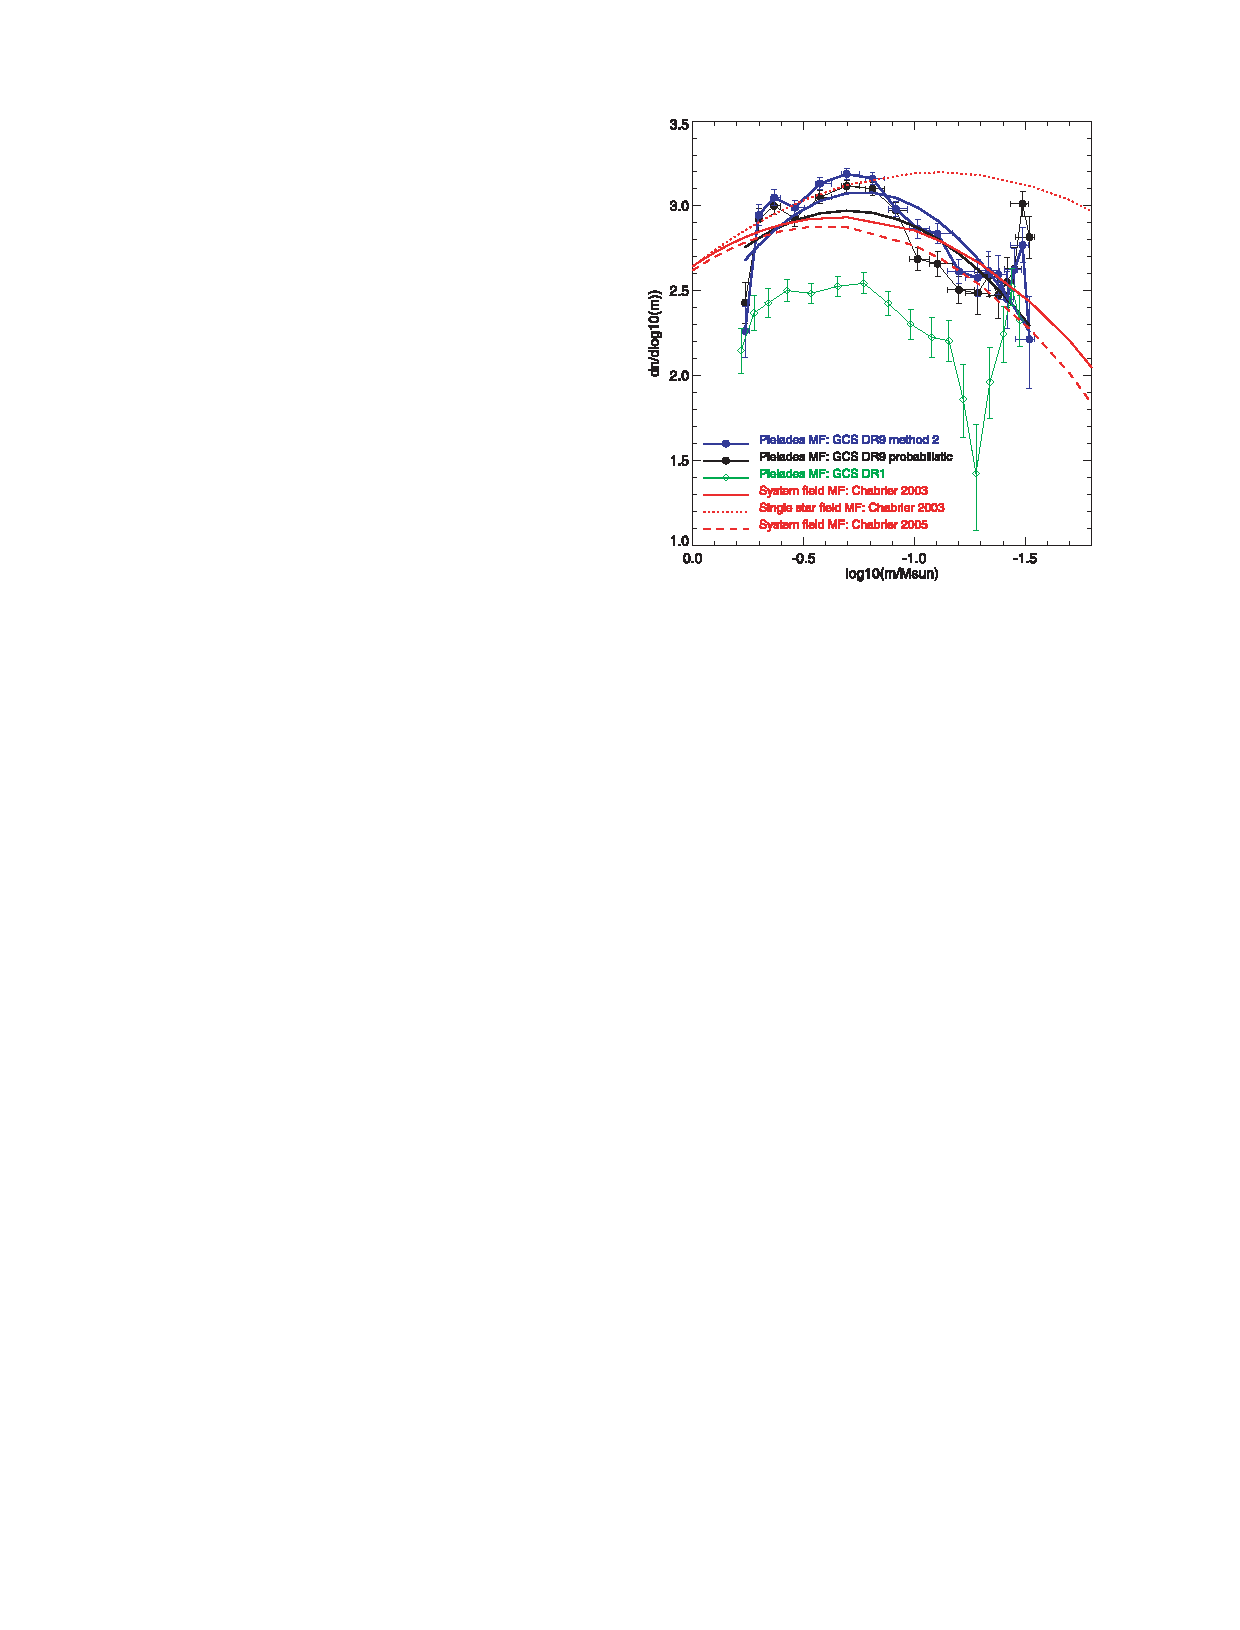
\includegraphics[height=8cm]{background/Figures/F9b_Lodieu2012.pdf}
\caption{Pleiades present day mass distribution from \citet{Lodieu2012}. GCS stands for Galactic Cluster Survey. The first and last two points must be treated with caution due to saturation and contamination at the bright and faint ends, respectively. Reproduced from Figure 9 of \citet{Lodieu2012}, \textit{\usebibentry{Lodieu2012}{Title}}, \usebibentry{Lodieu2012}{Journal}, Vol. \usebibentry{Lodieu2012}{Volume}.}
\label{fig:massLodieu}
\end{center}
\end{figure}

\begin{figure}[ht!]
\begin{center}
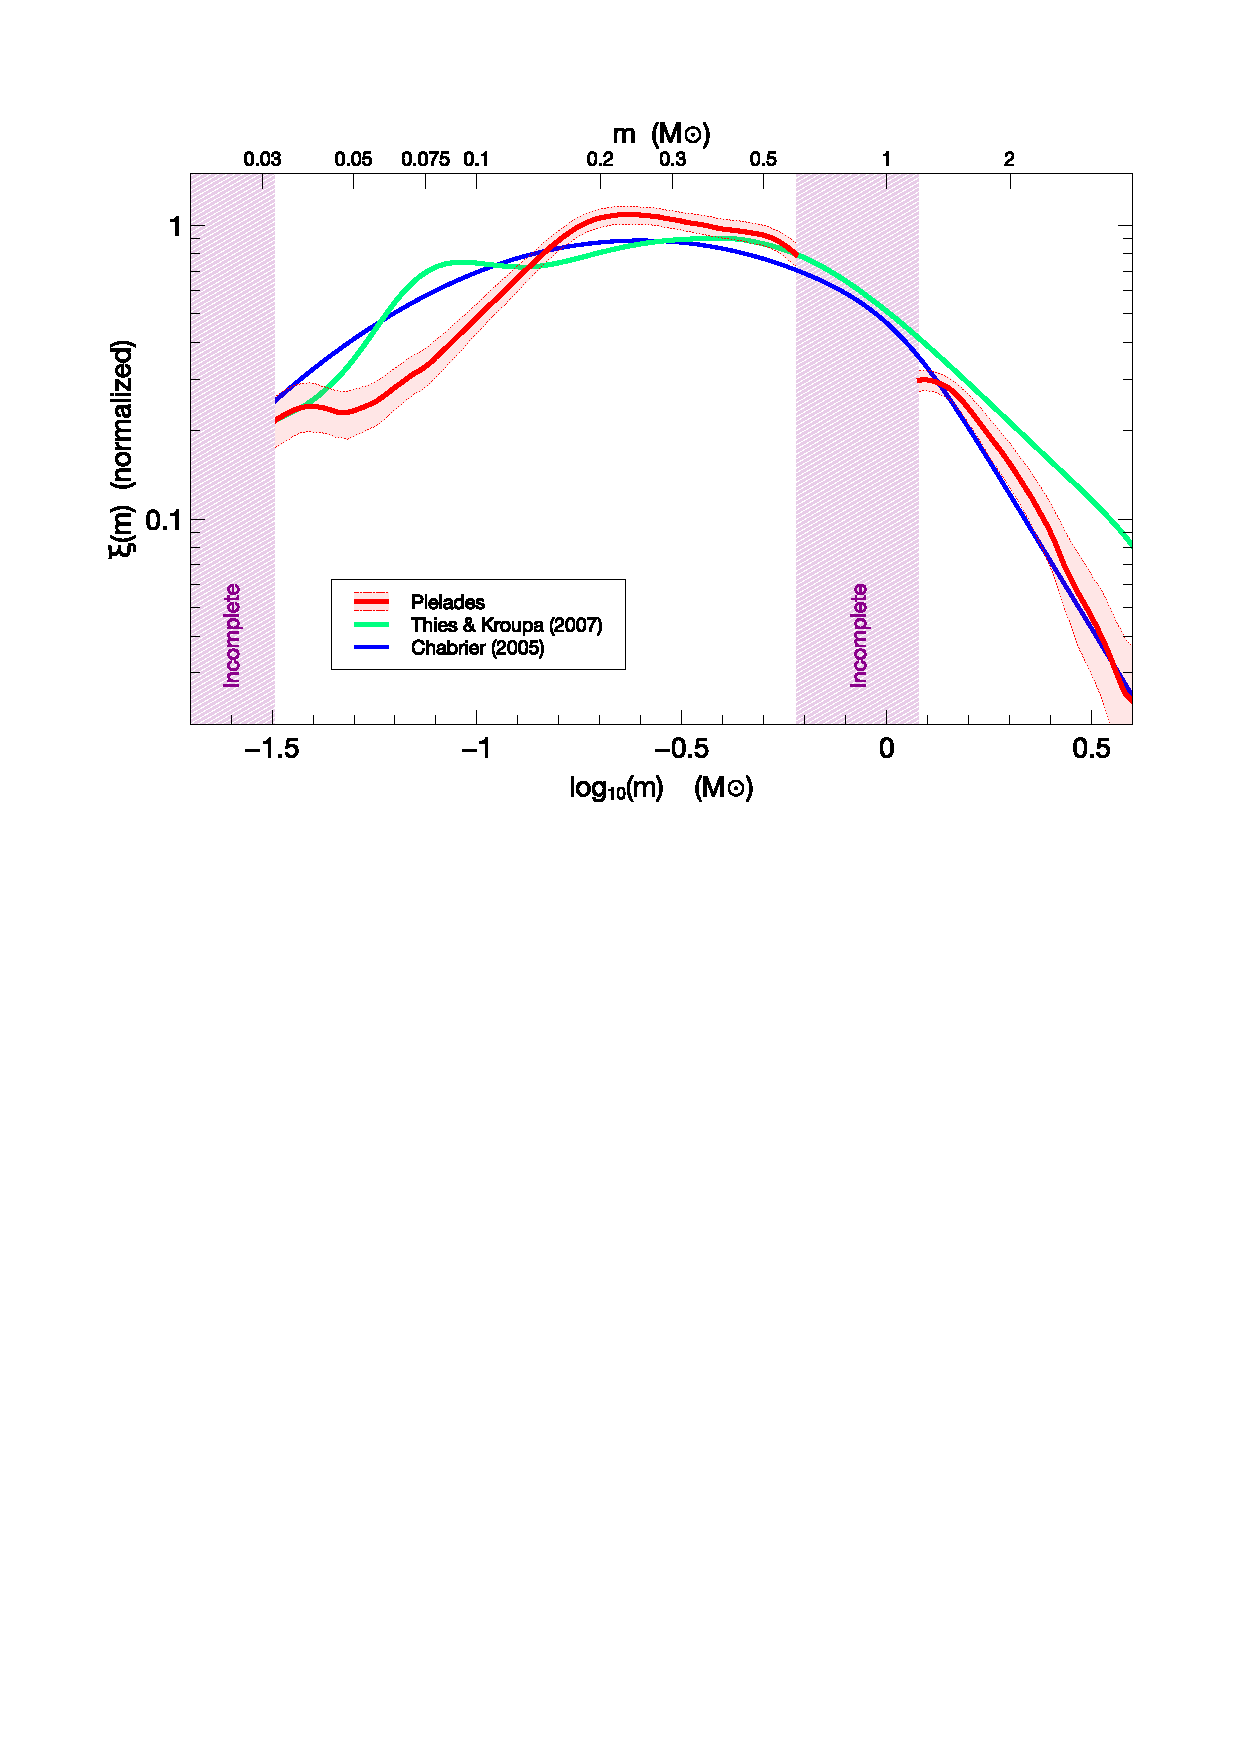
\includegraphics[height=8cm]{background/Figures/F9_Bouy2015.pdf}
\caption{Pleiades present day mass distribution  from \citet{Bouy2015} (red). \glspl{imf} from \citet{Chabrier2005}(blue) and \citet{Thies2007} (green) are also shown. Reproduced from Figure 9 of \citet{Bouy2015}, \textit{\usebibentry{Bouy2015}{Title}}, \usebibentry{Bouy2015}{Journal}, Vol. \usebibentry{Bouy2015}{Volume}.}
\label{fig:massBouy}
\end{center}
\end{figure}

\subsection{Total mass of the cluster}
Before ending this section I present a (non exhaustive) summary of the studies that provided an estimate of the total mass of the cluster.

The first record I found of the cluster total mass is that of \citet{1938AJ.....47...25T}. He estimated a total mass of $260 \,M_{\odot}$ assuming virial equilibrium. He also computed $200 \,\mathrm{M_{\odot}}$ using the Eddignton's mass-luminosity relation for objects brighter than $15$ mag in the visual band.

The subsequent works continue to report higher masses. \citet{1956MNRAS.116..296W} estimated a total mass of $337 \,\mathrm{M_{\odot}}$ using a polytrope model fitted to Hertzsprung's catalogue. He then mentions that taking into account Trumpler's data, the total mass should be about $500\,M_{\odot}$. 

\citet{Limber1962} computed the total mass in two ways. In the first one he assumed the cluster was virialised and obtained a mass of $900 \,M_{\odot}$. Using the luminosity function he estimated the lower limit to the total mass in $760 \,\mathrm{M_{\odot}}$. 

\citet{1970AJ.....75..563J} measured $470\,\mathrm{M_{\odot}}$ and $690\,\mathrm{M_{\odot}}$ using the luminosity distribution and the virial theorem, respectively. 

Later, \citet{1980IAUS...85..157V}  determined a total mass of $2000 \,\mathrm{M_{\odot}}$ using the virial theorem, a mean individual mass of $2\,\mathrm{M_{\odot}}$, and a velocity dispersion of $0.7\,\mathrm{km \cdot s^{-1}}$ in each spatial direction. 

\citet{1995JKAS...28...45L} measured $700 \,\mathrm{M_{\odot}}$ using the luminosity distribution and a mass-luminosity relation. 

\citet{Pinfield1998} fitting a King profile to the \gls{psd} of the cluster members obtained $735\,\mathrm{M_{\odot}}$. 

\citet{Adams2001} counting individual masses of candidate members within $5.5^{\circ}$ obtained a total mass of $690 \,\mathrm{M_{\odot}}$. 

\citet{Converse2008} found $820 \,\mathrm{M_{\odot}}$ after adding the individual masses of 1245  candidate members of \citet{Stauffer2007}. To obtain these masses they  transformed the $K$ and $I-K$ magnitude and colour into masses using the mass-luminosity relation given by the theoretical isochrone models of \citet{1998A&A...337..403B}. Later, \citet{Converse2010} redid their analysis and found the total mass to be $870\pm35\,\mathrm{M_{\odot}}$.

%\section{The current dynamical scenario}
%The most important sources of gravitational interactions affecting individual objects are due to: other individual objects (like for example close encounters or binary interactions), the ensemble of individual objects (the potential of the cluster itself or its momentum), other ensembles of objects (interactions with other clusters or molecular clouds) and, the galactic potential (perturbations due to the disk, resonances, arms).
%
%\subsection{Pleiades time-scales}
%Pinfield equation 13 and 14

\section{The Pleiades DANCe DR2}
\label{sect:DR2}

The \glsfirst{ddr2} contains astrometric (stellar positions and proper motions) and photometric ($ugrizYJHK_s$) measurements for 1,972,245 objects. As explained in Chapter 1, the \gls{dance} data set has an heterogenous origin, which can be observed in Fig. \ref{fig:originDANCeDR2} where the patchy pattern arise from the combination of several surveys. The interested reader can find more the details of this data set and its processing on \citet{Bouy2013}. Here, I briefly summarise its properties. Table \ref{tab:DR2properties} contains the basic statistics for the observables, while Table \ref{tab:DR2uncertainties} does it for the uncertainties. As an example, Fig. \ref{fig:pmuncert} shows the proper motions uncertainties as a function of the $i$ magnitude.

\begin{figure}[ht!]
\begin{center}
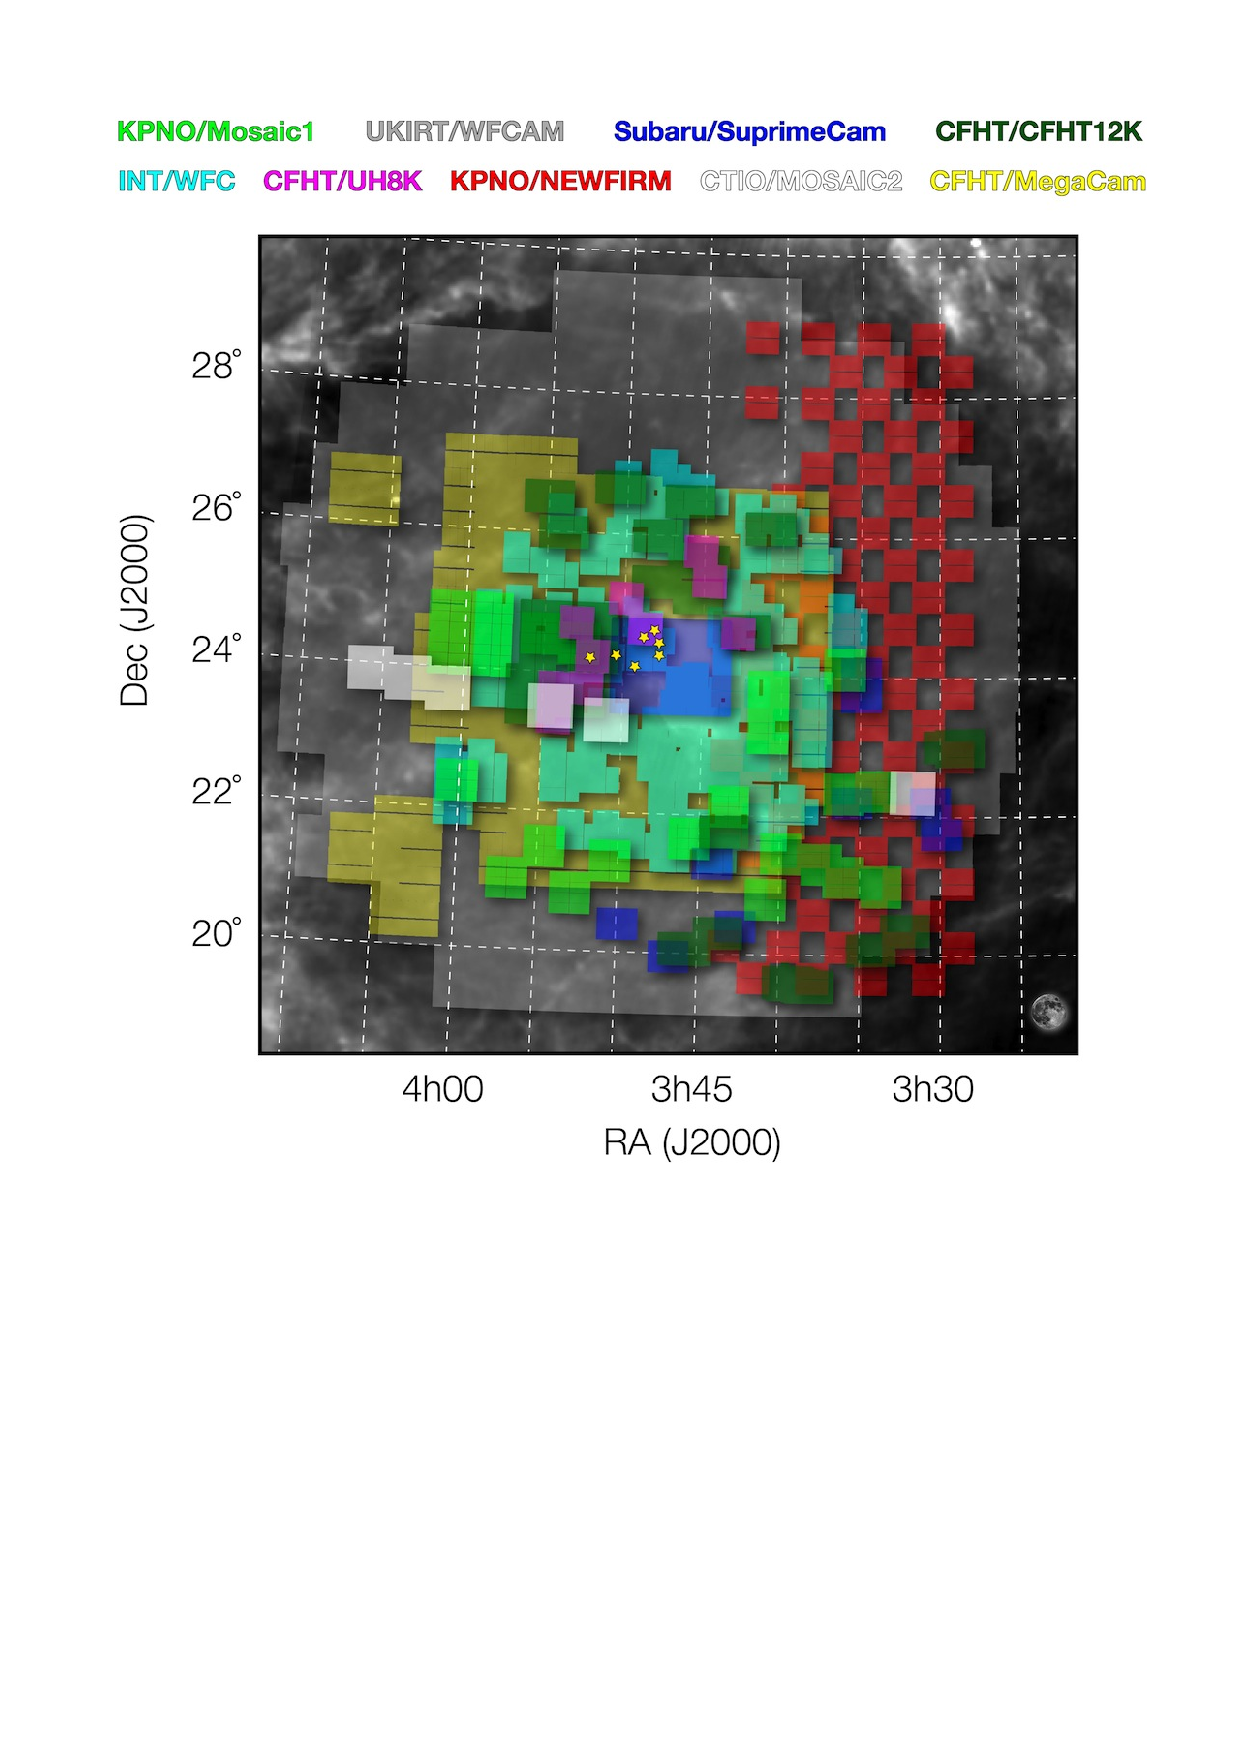
\includegraphics[width=\textwidth]{background/Figures/F1_Bouy2013.pdf}
\caption{Patchy composition of the \gls{ddr2}. The moon shows the scale, and the yellow stars correspond to the central brightest objects of the Pleiades cluster. As can be seen, the UKIDSS (UKIRT) survey provides the most homogeneous and extended coverage. Reproduced from Figure 1 of \citet{Bouy2013}, \textit{\usebibentry{Bouy2013}{Title}}, \usebibentry{Bouy2013}{Journal}, Vol. \usebibentry{Bouy2013}{Volume}.}
\label{fig:originDANCeDR2}
\end{center}
\end{figure}

\begin{table}[htdp]
\caption{Summary of the \gls{ddr2}.}
\begin{center}
\begin{tabular}{|c|c|c|c|c|c|c|c|}
\hline
Observable & Min. & 1st. Qu. & Median & Mean & 3rd. Qu. & Max. & NA's \\
\hline
\hline
RA [deg]&51.23 & 55.40 & 57.35 & 57.26 & 59.01 & 62.94 & 0\\
Dec. [deg] &19.12 &22.47 & 24.32 & 24.27  & 25.95 & 29.69 &0\\
$\mu_{\alpha} [mas\cdot yr^{-1}]$&-99.998& -6.060& -1.645& -1.240&3.401&99.996&0\\
$\mu_{\delta} [mas\cdot yr^{-1}]$&-99.997& -2.835&  2.548&  1.976&  7.017&99.989&0\\
u [mag]&13.6&20.4 &22.0 &21.6&23.3&25.2&1756374\\
g [mag]& 9.4   &19.6   &22.1   &21.1   &23.3   &25.5 &1492564\\
r [mag] &  8.4  &17.6   &21.3   &20.3   &22.6   &25.1   &1222853\\
i [mag] &  7.5  &20.0  &21.6  &21.0  &22.7  &25.5  &820861\\
z [mag]&11.2  &17.9  &19.3  &18.9  &20.2  &25.0  &697412\\
Y [mag]& 8.3  &17.2  &18.5  &18.1  &19.4  &24.2  &688144\\
J [mag]& 2.8  &16.7  &17.9  &17.5  &18.8  &23.1  &645469\\
H [mag]& 2.0  &16.1  &17.3  &16.9  &18.1  &20.9  &653682\\
$K_s$ [mag]& 1.8 &16.0&  17.0  &16.7  &17.7  &23.8  &561745\\
\hline
\end{tabular}
\end{center}
\label{tab:DR2properties}
\end{table}%

\begin{table}[ht!]
\caption{Uncertainties of the \gls{ddr2}.}
\begin{center}
\begin{tabular}{|c|c|c|c|c|c|c|c|}
\hline
Observable & Min. & 1st. Qu. & Median & 3rd. Qu. & Max. &Mean\\
\hline
\hline
RA [deg]&8.900e-08 &9.270e-07&1.933e-06&4.037e-06&2.156e-02&3.173e-06\\
Dec. [deg] &8.900e-08&9.270e-07&1.932e-06&4.037e-06&2.156e-02&3.173e-06\\
$\mu_{\alpha} [mas\cdot yr^{-1}]$&2.01e-01 &1.89e+00& 4.35e+00& 1.00e+01& 1.49e+22&3.99e+16\\ 
$\mu_{\delta} [mas\cdot yr^{-1}]$&1.92e-01 &1.89e+00 &4.35e+00 &1.00e+01 & 4.71e+09&1.42e+04\\
u [mag] &3.73e-04& 8.07e-03& 3.06e-02& 8.56e-02& 2.17e-01&5.48e-02\\
g [mag] &1.72e-01 & 1.02e-02&  3.90e-02 & 7.90e-02 & 1.82e+00&5.34e-02\\
r [mag] & 2.83e-04 & 1.54e-02& 4.88e-02 &1.04e-01& 1.42e+00&6.34e-02\\
i [mag] & 4.04e-04 & 9.03e-03&  2.73e-02& 5.85e-02& 2.40e+00&4.37e-02\\
z [mag] & 6.49e-04& 5.62e-02& 9.16e-02& 1.85e-01& 3.12e+00&1.34e-01\\
Y [mag] & 3.00e-02& 5.21e-02& 6.50e-02& 1.03e-01& 9.01e+00&8.56e-02\\
J [mag] & 1.60e-02& 5.24e-02& 6.66e-02& 1.04e-01& 8.89e+00&8.57e-02\\
H [mag] & 1.40e-02& 5.28e-02& 7.04e-02& 1.10e-01& 1.00e+01&8.85e-02\\
$K_s$[mag]&1.40e-02& 5.75e-02& 8.17e-02& 1.32e-01& 3.88e+01&1.04e-01\\
\hline
\end{tabular}
\end{center}
\label{tab:DR2uncertainties}
\end{table}%

\begin{figure}[ht!]
\begin{center}
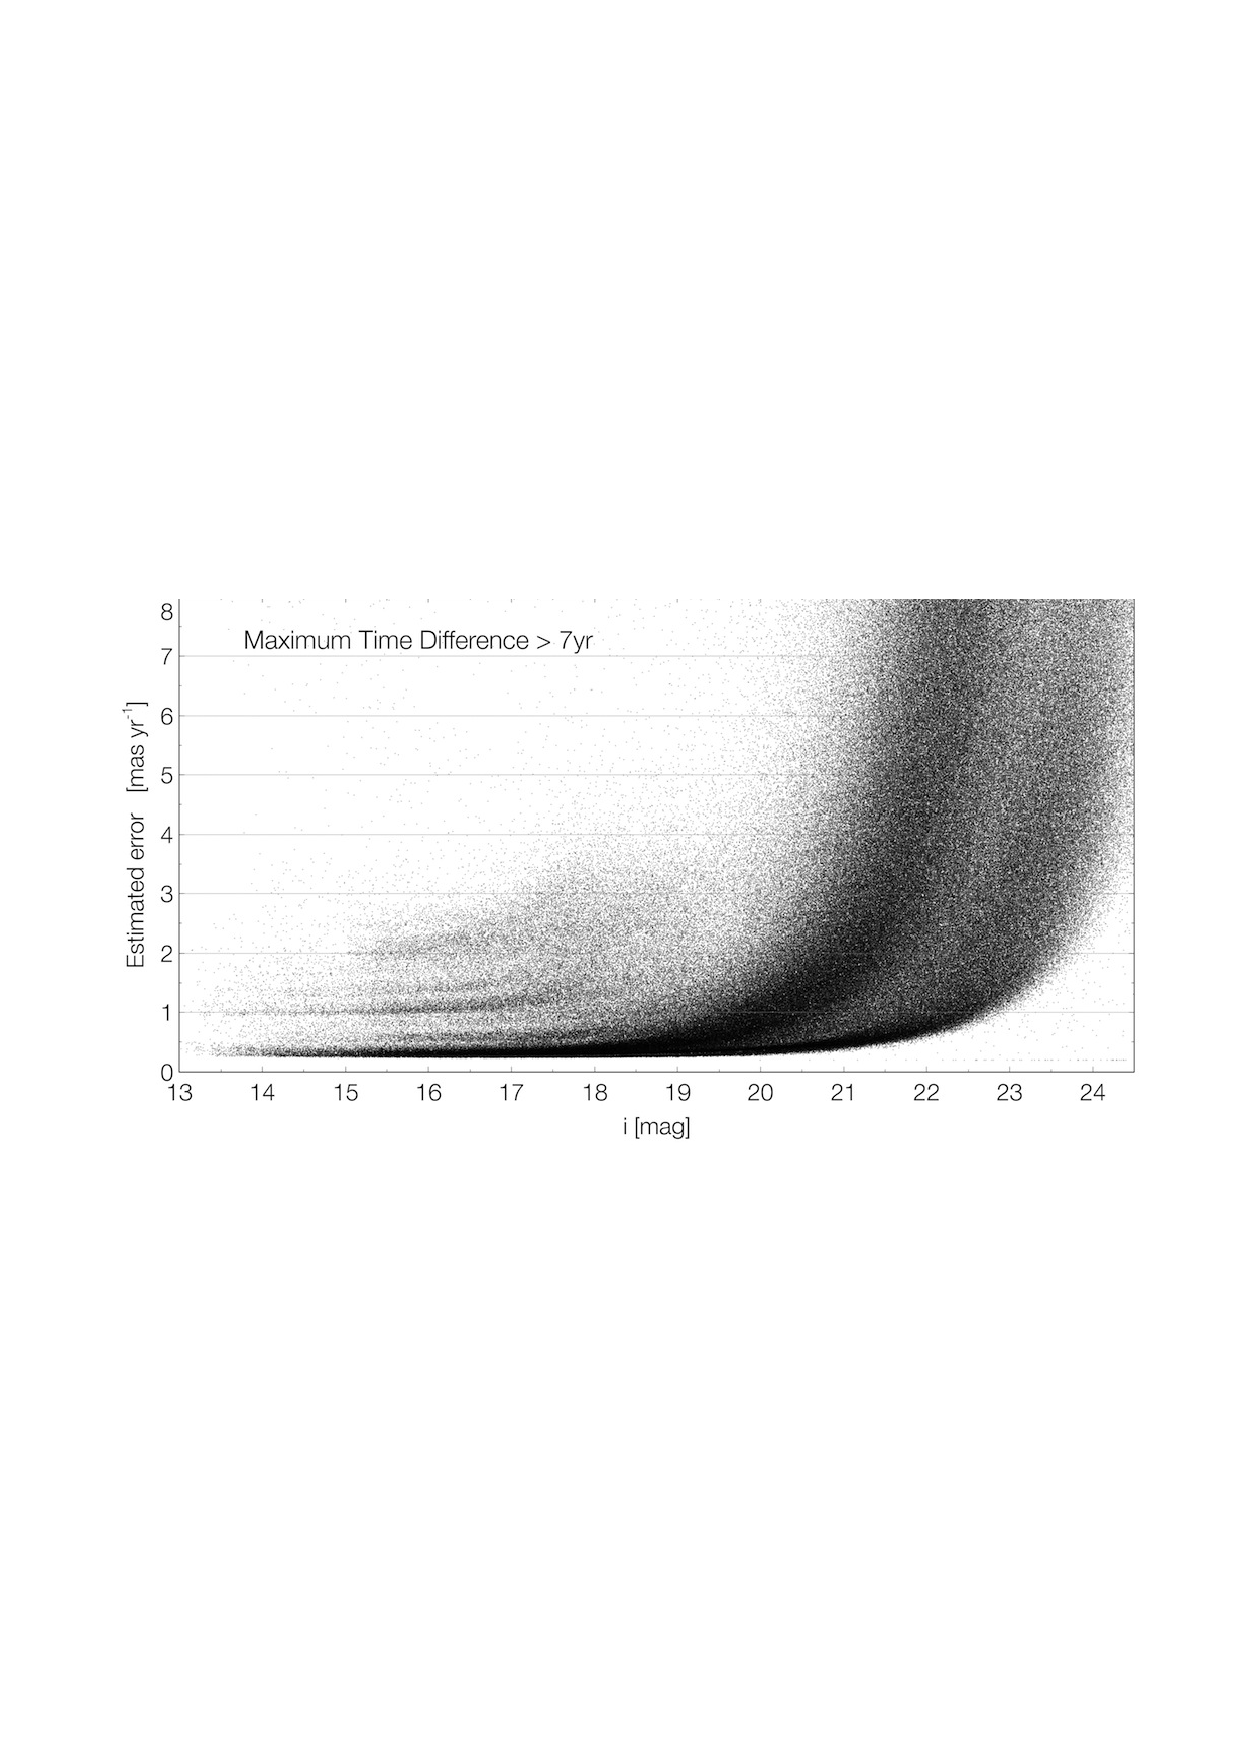
\includegraphics[height=8cm]{background/Figures/F12_Bouy2013.pdf}
\caption{Proper motion uncertainty as a function of the photometric magnitude in the $i$ band. Reproduced from Figure 12 of \citet{Bouy2013}, \textit{\usebibentry{Bouy2013}{Title}}, \usebibentry{Bouy2013}{Journal}, Vol. \usebibentry{Bouy2013}{Volume}.}
\label{fig:pmuncert}
\end{center}
\end{figure}

\subsection{Missing values}
In the \gls{ddr2}, missing values occur only in the photometric measurements (see Table \ref{tab:DR2properties}), with the bluer bands being the most affected. As expected, the probability distribution of sources with missing values is not uniform. Missing values occur with higher probability at the faintest end of the photometric distributions ($\sim 18$ mag in $J,H$ and $K_s$ bands). Figure \ref{fig:NAsDDR2} shows the distribution of objects having at least a missing entry as a function of the band or bands that were actually observed. As mentioned, the vast majority of these objects occur at the faint end, close to the sensitivity limit of the survey. It coincides with the sensitivity limits of the UKIDSS Galactic Cluster Survey \cite[$Y\sim 20.3$, $J\sim19.5$, $H\sim K_s\sim18.6$ according to][]{2007MNRAS.379.1599L}, which provides the deepest photometry in the \gls{ddr2}. In this Figure, the bumps at the bright and middle ranges arise due to the mixing of surveys. The first bump corresponds to the survey carried out by \citet{Bouy2015}. As mentioned in their Appendix A, due to saturation, the $Y$ band photometry was limited to objects fainter than $\sim 13$ magnitude. Thus, they complemented the Pleiades \gls{dance} catalogue with shallow $Y$ band photometry in the magnitude range of 8 to 14 magnitudes but only for 40 candidate members of \citet{Stauffer2007} and their surrounding objects \cite[see][for more details]{Bouy2015}. Thus, the large amount of missing $Y$ values in the 8 to 14 mag range of Fig. \ref{fig:NAsDDR2} come from those objects not observed by these authors. The second bump at the middle range is slightly fainter than the sensitivity limits of the 2MASS survey ($J\sim 16.4$, $H\sim15.5$ and $K_s \sim 14.8$, see Section 6.2 of the Explanatory Supplement to the 2MASS All Sky Data Release\footnote{\url{https://www.ipac.caltech.edu/2mass/releases/allsky/doc/sec6_2.html}}), which indicates that it comes from the mixing of the 2MASS and UKIDSS surveys. Due to the different spatial resolutions, some objects are detected in 2MASS and not in UKIDSS and vice versa. The missing $Y$ band values come from objects observed only by 2MASS.

\begin{figure}[ht!]
    \centering
    \begin{subfigure}[t]{0.45\textwidth}
        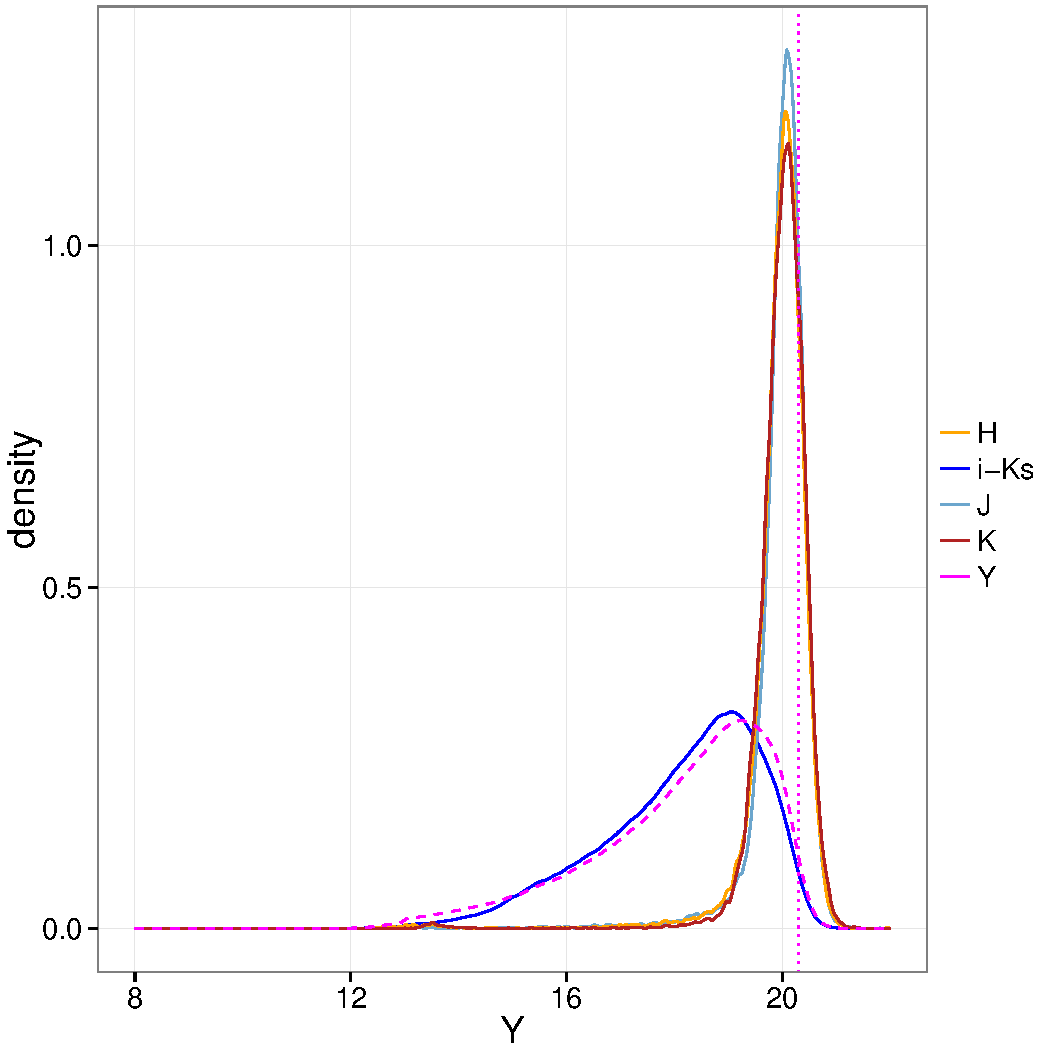
\includegraphics[page=1,height=6cm]{background/Figures/MissingDistributionsDDR2.pdf}
    \end{subfigure}
    \begin{subfigure}[t]{0.45\textwidth}
      \includegraphics[page=2,height=6cm]{background/Figures/MissingDistributionsDDR2.pdf}
    \end{subfigure}
     \begin{subfigure}[t]{0.45\textwidth}
      \includegraphics[page=3,height=6cm]{background/Figures/MissingDistributionsDDR2.pdf}
    \end{subfigure}
     \begin{subfigure}[t]{0.45\textwidth}
      \includegraphics[page=4,height=6cm]{background/Figures/MissingDistributionsDDR2.pdf}
    \end{subfigure}
\caption{Density distributions in $Y,J,H$ and $K_s$ bands for \gls{ddr2} objects with missing values in the other bands. For comparison, the distribution of observed objects is also shown with a dashed line. The majority of the missing value objects are located at the faint end of the magnitude distributions ($Y \sim 20$, $J \sim 19$, $H\sim18.5$, and $K_s \sim 18$). A non negligible fraction of missing  $Y$ band photometry is at the bright end ($J,H,K_s \sim 8 - 14$ mag), and in the middle range of 13 to 16 magnitudes. See text for details.}
\label{fig:NAsDDR2}
\end{figure}

\begin{figure}[ht!]
    \centering
    \begin{subfigure}[t]{0.45\textwidth}
        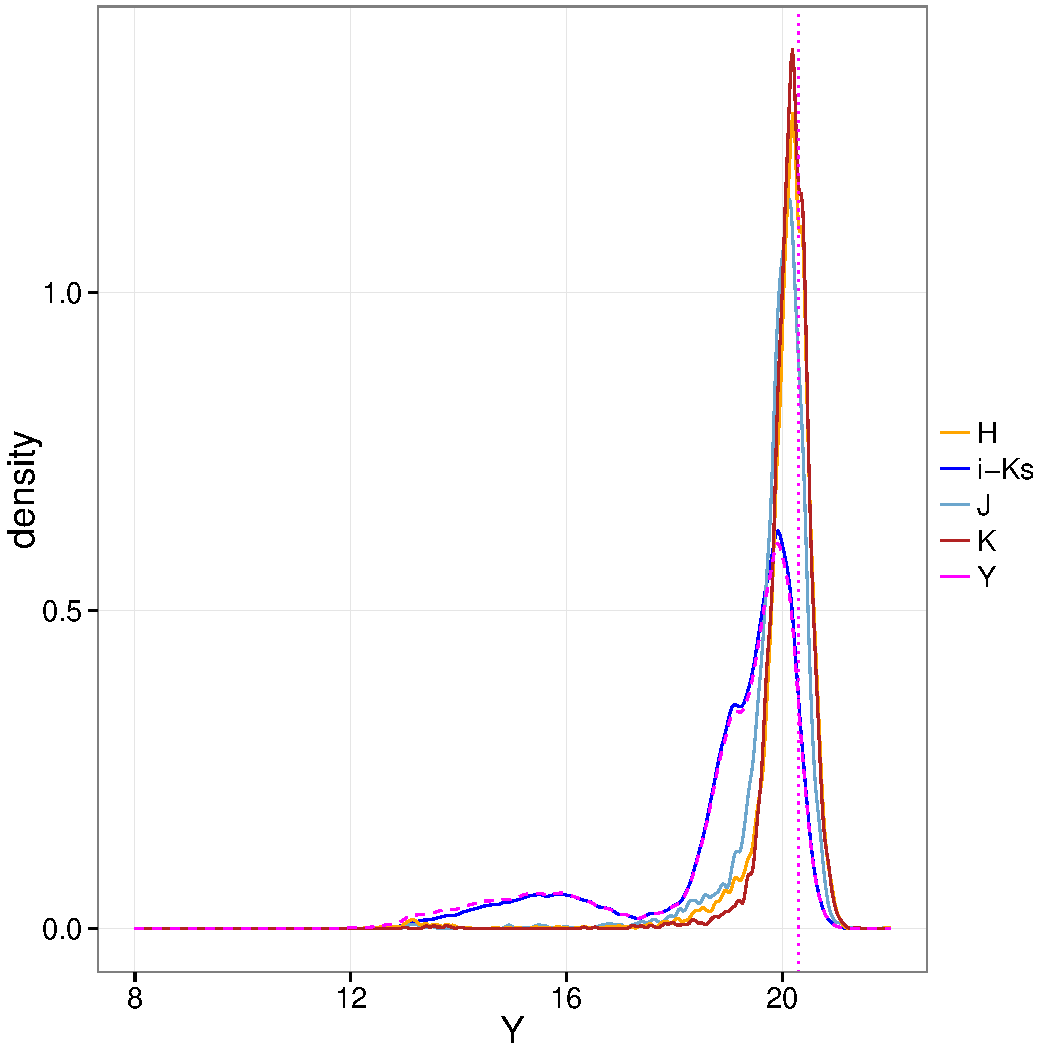
\includegraphics[page=1,height=6cm]{background/Figures/MissingDistributions.pdf}
    \end{subfigure}
    \begin{subfigure}[t]{0.45\textwidth}
      \includegraphics[page=2,height=6cm]{background/Figures/MissingDistributions.pdf}
    \end{subfigure}
     \begin{subfigure}[t]{0.45\textwidth}
      \includegraphics[page=3,height=6cm]{background/Figures/MissingDistributions.pdf}
    \end{subfigure}
     \begin{subfigure}[t]{0.45\textwidth}
      \includegraphics[page=4,height=6cm]{background/Figures/MissingDistributions.pdf}
    \end{subfigure}
\caption{Density distributions in $Y,J,H$ and $K_s$ bands of \gls{rdr2} for objects with missing values in the other bands. For comparison, the distribution of observed objects is also shown with a dashed line. The features are similar to those in Fig. \ref{fig:NAsDDR2}. The small differences between the two figures come from the fact that the \gls{rdr2} is not a random sample of the \gls{ddr2}.}
\label{fig:NAs}
\end{figure}


\subsection{Completeness limits}
\label{sect:ddr2_completeness}

EXPLAIN THE ASSUMPTION ABOUT THE POWER LAW IN THE NUMBER OF SOURCES AND THAT NO MODEL IS USED TO DETERMINE THIS COMPLETENESS.
The completeness limits of the derived luminosity distributions are acquired as follows. Since the \gls{bhm} methodology prescribes the \emph{true} photometric quantities based on the \emph{true} colour index \gls{ci}. Then, the completeness limits of the \gls{ci} distribution dictate those of the luminosity distributions. 

\citet{Bouy2015} mention that, due to the heterogeneous origins of the \gls{ddr2} data set, the spatial coverage and sensitivity of the survey is also not homogeneous. To remedy this issue, they identify a region with complete spatial coverage, the inner three degrees of the cluster (see Fig. \ref{fig:originDANCeDR2}). Then, they restricted their photometric analysis to this spatially complete region. 

Restricting their sample of candidate members to this inner region results in a sample of candidate members that is spatially biased. If any dynamical process has been set on the cluster such that the mass distribution of its members is not uniformly distributed in the space, then a spatial cut in a sample of candidate members will result in a bias on the mass distribution. One of such dynamical process is the mass segregation, which, as suggested by \citet{Adams2001} may have happen in the Pleiades cluster. As proven in Section \ref{sect:lumsegregation}, there is strong evidence in favour of luminosity segregation in the Pleiades, at least in the $J$ band.

Thus, to avoid such biases, I assume that the UKIDSS survey, which is the most profound from among the contributions to the \gls{ddr2} data set, provides the homogeneous spatial and sensitivity coverage at faint magnitudes (see Fig. \ref{fig:originDANCeDR2}). This survey thus provides the upper completeness limits, which are essentially those reported in the Appendix A of \citet{Bouy2015}, $i\sim23$ mag and $K_s\sim18$ mag.

Since we are interested in the completeness limits of the $\gls{ci}$, and this equals $i -K_s$, then its completeness limits are defined by those of $i$ and $K_s$ together. In Fig. \ref{fig:completeness}, I show the $K_s$ and $i$ kernel density estimate computed using all sources in the \gls{ddr2}. As can be seen from this Figure, the point with maximum density, which corresponds to $i=21.4$ mag and $K_s=18.1$ mag, should be used to set the upper completeness limits. Notice that, due to the use of the two dimensional density, the upper completeness limit in $i$ is reduced with respect to that of the univariate $i$ distribution. This density shows a sharp decline at bright magnitudes, probably due to saturation of the detectors. To be conservative, I choose $i=13.2$ mag and $K_s=11.0$ mag as the lower completeness limits.

\begin{figure}[htbp]
\begin{center}
\resizebox{\hsize}{!}{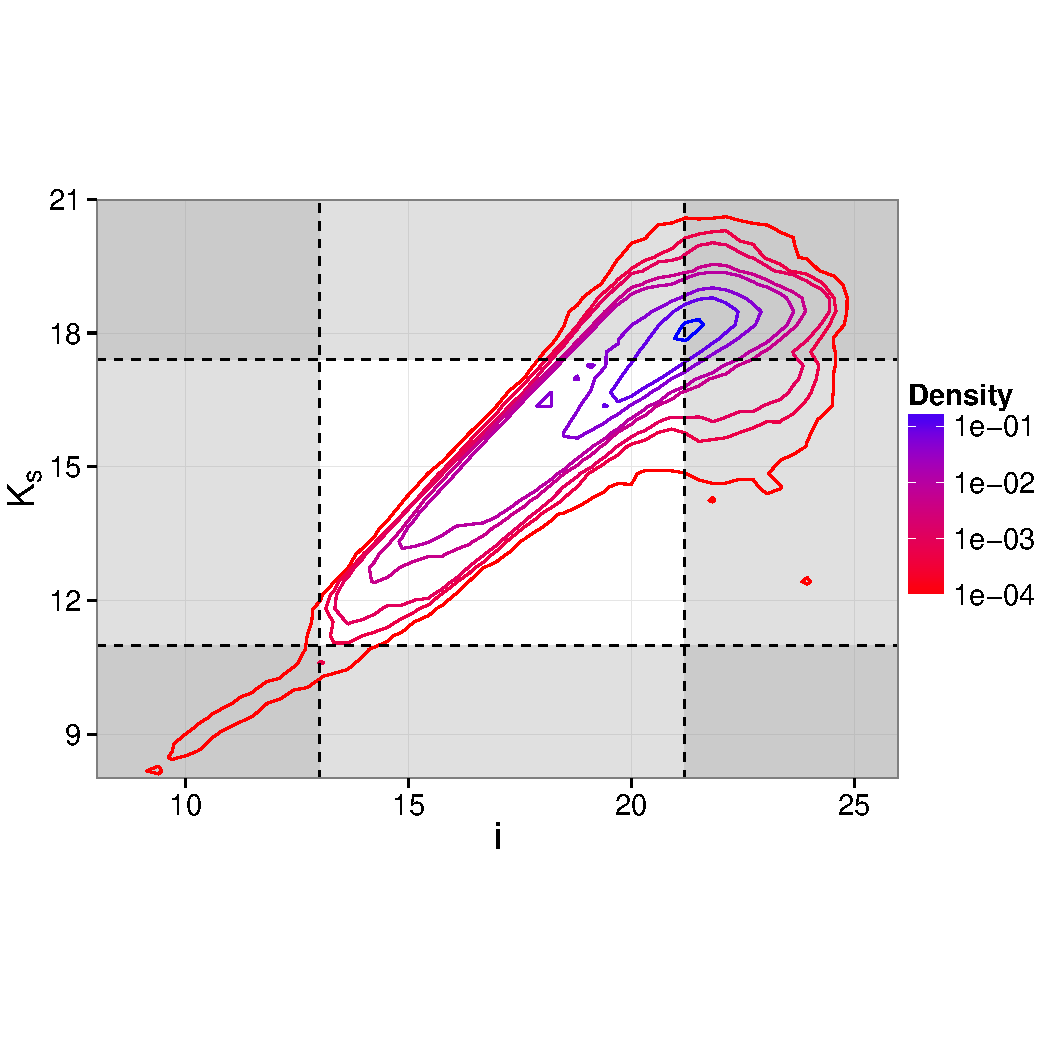
\includegraphics[width=0.8\textwidth]{background/Figures/Density-Kvsi.pdf}}
\caption{Density of all \gls{ddr2} sources in $K_s$ and $i$ magnitudes. Lines show the chosen completeness limits, $13.2<i<21.4$ mag and $11<K_s<18.1$ mag. The grey area is considered incomplete. Reproduced from Figure 9 of \citet{Olivares2017},\textit{\usebibentry{Olivares2017}{Title}}, \usebibentry{Olivares2017}{Journal}, Vol. \usebibentry{Olivares2017}{Volume}.}
\label{fig:completeness}.
\end{center}
\end{figure}

\subsection{Selection of observables}
\label{sect:RF-2}
\sloppy
The \gls{ddr2} contains the positions R.A., Dec. (in the following $\alpha$ and $\delta$), proper motions, $\mu_{\rm{R.A.}},\mu_{\rm{Dec.}}$, and photometric $ugrizYJHK_s$ bands, of almost two million sources on the vicinity of the Pleiades clusters. Although these 13 observables carry information valuable to discriminate cluster members from field objects, not all of them do it in the same way. A detailed analysis of the capacity of the previous set of observables (except the stellar postions) to discriminate between cluster members and field population is present in the work of \citet{Sarro2014}. These authors use random forest to select the observables that were the most discriminant. They find that the observables of  proper motions ($\mu_{R.A.},\mu_{Dec.}$) and the photometric bands $rizYJHK_s$ are the most discriminants. 

However, since most the objects with a missing $r$ band occur at the faint end of the cluster sequence, \citet{Sarro2014} train their model in two stages. In the first stage, they use all literature candidate members with observed $r$ band. In the second stage, they discard the $r$ band observations and continue training their model with objects in which the $r$ band was missing.  In a subsequent analysis using roughly the same methodology, \citet{Bouy2015} skipped the first training stage and worked only with the RF-2, which also excludes the $z$ band.

Therefore, in the present work I use as a reference set the the proper motions, $\mu_{\alpha},\mu_{\delta}$, the photometric bands $Y,J,H,K_s$, and the colour index $i-K_s$, with the addition of the stellar positions  $\alpha$ and $\delta$. This decision roots in two key aspects. First,  \citet{Sarro2014} prove that this observables (excluding the stellar positions) are amongst the most discriminant ones. Second, this set corresponds to the one used by \cite{Bouy2015}, thus, it will enable us to perform a direct comparison and validation with their results. 

However, there is a subtle difference between the set of observables used by \cite{Bouy2015} and the ones use in the present work. While here I use the $Y$ band alone, \citet{Bouy2015} use the colour index $Y-J$. Originally, I tested the methodology with this $Y-J$ colour index, however, the contamination resulting from the use of the $Y$ gets reduced with respect to that of the $Y-J$ colour index. I interpret this situation as resulting from at least two points. First, the $Y-J$ colour index does not convey information for the sequence of equal-mass binaries, thus reduces the capacity to identify these objects. Second, the width of the cluster sequence in the $Y-J$ vs. $i-K_s$ colour-colour diagram varies greatly across $i-K_s$ when compared to the relatively stable width of the cluster sequence in the the $Y$ vs $i-K_s$ \gls{cmd}. This effect can be observed in Figure \ref{fig:Y-JvsY}, where the candidate members of \citet{Bouy2015} (blue dots) are depicted, together with the \gls{rdr2} density, in the colour-colour diagram $Y-J$ vs. $i-K_s$, and the  \gls{cmd} $Y$ vs $i-K_s$. Since the current version of the photometric model describes the cluster sequence with a constant width across the $i-K_s$ colour index (details are shown in Section \ref{sect:cluster_ph}), then the use of $Y-J$ results in larger contamination in those regions where the clusters sequence is narrower than the average. Future steps will be take to include more colour indices in the reference set of observables.

\begin{figure}[htp!]
\begin{center}
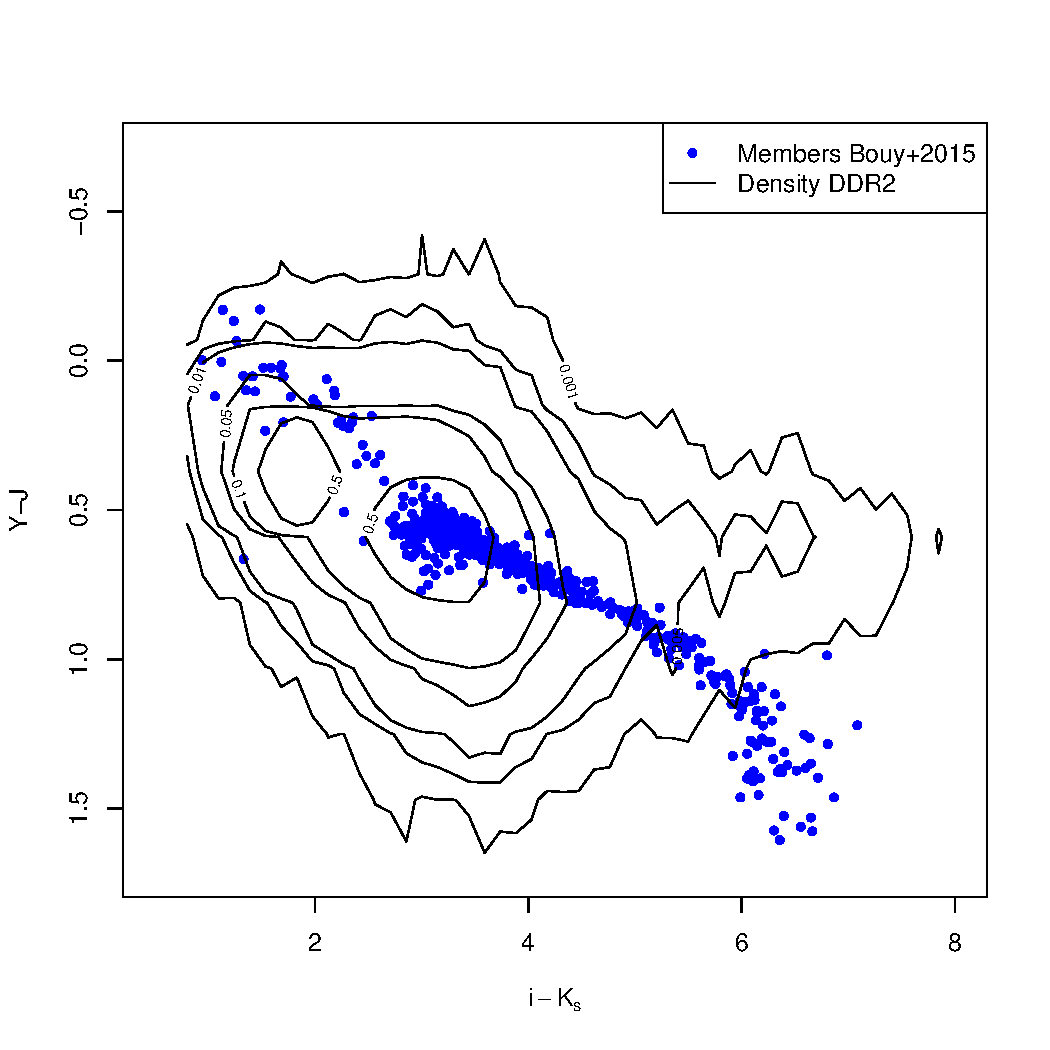
\includegraphics[page=1,width=0.47\textwidth]{background/Figures/Y-J.pdf}
\includegraphics[page=2,width=0.47\textwidth]{background/Figures/Y-J.pdf}
\caption{Candidate members of \citet{Bouy2015}, blue dots, together with the density of the \gls{rdr2} data set, black contours, in the colour-colour  diagram $Y-J$ vs. $i-K_s$ (left) and \gls{cmd} $Y$ vs $i-K_s$ (right).}
\label{fig:Y-JvsY}
\end{center}
\end{figure}
 

 
Concerning the stellar positions $\alpha$ and $\delta$, neither \citet{Bouy2015} nor \citet{Sarro2014} use them in their analyses. Thus, I will independently analyse the: i) the kinematic and photometric distributions of the cluster population, and ii) the \gls{psd}. This decision roots in the following reasons.

First. To fulfil the objective of the \gls{dance} project (see Section \ref{sect:DANCeproject}), the inventory of kinematic and photometric distributions of the \glspl{nyc} must be obtained with an homogenous methodology. The \gls{dance} \gls{nyc} targets (see Tables \ref{tab:maintargets} and \ref{tab:secondarytargets}) do not share similar projected spatial density profiles; while Taurus, Ophiucus and the Trapezium are extended \cite[see for example][]{simon1997}, the Pleiades is almost radially symmetric \citep{Raboud1998}. Thus, including the spatial information together with the proper motions and photometry would require completely different models for the \gls{psd} of different clusters. That would result in non-homogenous methodologies that would bias any comparison between the derived \gls{pdsmd} of these clusters.

{Second. To validate the results of the present work, which will be conducted in the Pleiades cluster, we must compare them with similar results under the most similar conditions. Since \citet{Bouy2015,Sarro2014} do not include the stellar positions in their observables, I do that as well. }

{Third. Almost all previous analyses of the Pleiades \gls{psd} use King profile (see Section \ref{sect:PSD}) without providing any further reason that its physical interpretability, which nevertheless remains a good one. Thus, we decided to perform a Bayesian model selection analysis to compare how well the common surface density profiles, included the King's one, reproduce the Pleiades \gls{psd}. The results of this analysis are in preparation and will be soon submitted to the $A\&A$ journal. }

As will be described in Section \ref{subsect:cluster}, the photometry is modelled by parametric series of cubic splines. I choose the \emph{true} \gls{ci} to be the parameter of these series. This colour allows the most one-to-one dependent-independent variable relations. This one-to-one relation can be seen in Figures \ref{fig:CI} and \ref{fig:otherCI}, where I show the colour-magnitude diagram of $K$ vs $i-K_s$ and $K$ vs colours $Y-K_s$, $J-K_s$, $H-K_s$, and $Y-J$, respectively.  This one-to-one relation is crucial to avoid degeneracies. Without it, two magnitudes could be described by the same colour index. Therefore a monotonic relation would not be valid. 

Thus, our photometric set of observables is made of $i-K_s, Y,J,H$ and $K_s$. 

\begin{figure}[ht!]
\begin{center}
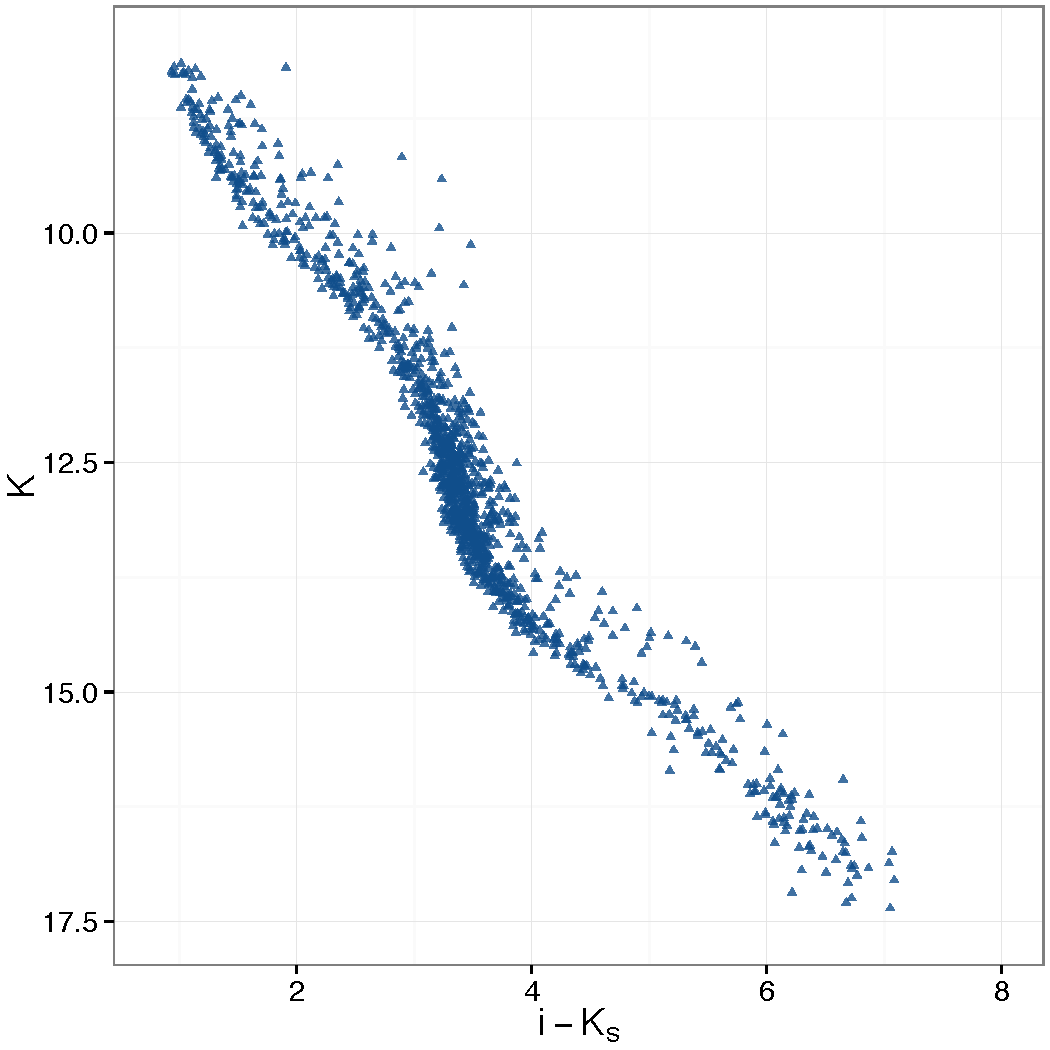
\includegraphics[page=1,height=8cm]{background/Figures/CIs.pdf}
\caption{$K_s$ vs $i-K_s$ CMD for the Pleiades candidate members of \citet{Bouy2015} with membership probability $>0.75$.}
\label{fig:CI}
\end{center}
\end{figure}

\begin{figure}[ht!]
    \centering
    \begin{subfigure}[t]{0.45\textwidth}
        \includegraphics[page=2,height=6cm]{background/Figures/CIs.pdf}
        \caption{}
        
    \end{subfigure}
    \begin{subfigure}[t]{0.45\textwidth}
      \includegraphics[page=3,height=6cm]{background/Figures/CIs.pdf}
        \caption{}
         
    \end{subfigure}
     \begin{subfigure}[t]{0.45\textwidth}
      \includegraphics[page=4,height=6cm]{background/Figures/CIs.pdf}
        \caption{}
         
    \end{subfigure}
     \begin{subfigure}[t]{0.45\textwidth}
      \includegraphics[page=5,height=6cm]{background/Figures/CIs.pdf}
        \caption{}
         
    \end{subfigure}
    \caption{CMD for the Pleiades candidate members of \citet{Bouy2015}  with membership probability $>0.75$. The magnitude $K_s$ is shown versus the colour indices: $Y-K_s$(a), $J-K_s$(b), $H-K_s$(c), and $Y-J$ (d).}
    \label{fig:otherCI}
\end{figure}


\subsection{Data preprocessing}
\label{sect:RDR2}
Since both photometry and proper motions carry crucial information for the disentanglement of the cluster population, we restrict the data set to only those objects with observed proper motions, and also at least two photometric entries in our photometric set ($i-K_s,Y,J,H,K_s$). {Objects with only one photometric entry, although theoretically could be included in the data set, are left aside due to computational reasons. Their treatment requires selection statements to choose between the univariate and multivariate computational libraries that proved to be computationally expensive.}

The previous restrictions exclude 22 candidate members of \citet{Bouy2015}, which only have one observed value in the photometry. For these particular objects, we compute their marginal proper motion membership probability a posteriori, once the parameters of the model were inferred. The mode and 16 and 84 percentiles of their membership probabilities are listed in Table \ref{tab:22excluded}. Only four of these 22 objects have membership probabilities below 0.5, which may indicate they are contaminants. Since these membership probabilities were computed using only the kinematic information, these four members could not be discarded as probable candidate members.

\textbf{In the following, whenever I mention the Pleiades candidate members of \citet{Bouy2015}, I refer to the 1988 objects in the \gls{ddr2} with \citet{Bouy2015} membership probabilities grater than 0.75, and with at least two observed values in the photometry.}

\begin{table}[htdp]
\caption{Membership probabilities of the 22 excluded candidate members of \citet{Bouy2015}.}
\begin{center}
\begin{tabular}{|c|c|c|c|}
\hline
ID DANCe & $P_{16}$ & Mode & $P_{84}$\\
\hline
\hline
J035106.55+211604.3 &0.751182& 0.7774335&    0.785560\\
J035057.42+240630.8 &0.792295& 0.8090186&   0.829541 \\
J034704.76+252249.8& 0.701193& 0.7319624 &   0.750745\\
J034725.80+250832.7 &0.789872& 0.8169538 &  0.827954 \\
J034437.44+250815.6 &0.762013& 0.7773114 &   0.798125\\
J035125.88+244738.6& 0.883488& 0.9007972 &  0.905823 \\
J034235.64+215029.7 &0.838538& 0.8662402 &  0.871439 \\
J034516.66+243432.1 &0.862284& 0.8666611 &   0.881004\\
J034926.12+235714.8& 0.852537& 0.8606685 &  0.866286 \\
J034920.60+244635.9 &0.923319& 0.9270399 &  0.935532 \\
J035300.63+233252.3 &0.762996& 0.7747163 &  0.781901 \\
J034606.52+235020.2& 0.928688& 0.9333306 &  0.940772 \\
J035040.89+245657.7 &0.509435& 0.5215143 &  0.530379 \\
J034845.33+233124.8 &0.260551& 0.2650812 &  0.275513 \\
J034713.67+234953.3& 0.814689& 0.8489593 &  0.855902 \\
J034546.48+234743.0 &0.897035& 0.9098442 &  0.912059 \\
J034548.95+235110.2 &0.933892& 0.9376429 &   0.945558\\
J035202.26+242148.1& 0.248011& 0.2649874 &   0.305949\\
J035313.22+235540.8 &0.518388& 0.5425345 &  0.553376 \\
J034425.60+244052.5 &0.581242& 0.5902633 &  0.602096 \\
J035518.38+245637.2& 0.198074& 0.2087989 &  0.252831 \\
J035418.93+252944.0& 0.366009& 0.3760922 &  0.386213 \\
\hline
\end{tabular}
\end{center}
\label{tab:22excluded}
\end{table}%


Furthermore, we restrict the lower limit of the \gls{ci} to the value of the brightest cluster member, \gls{ci}=0.8 in the \gls{ddr2} data set (\textbf{The actual value is \gls{ci}=0.93, see Table \ref{tab:rddr2_cluster}, but 0.8 was chosen conservatively to include the uncertainty}). We do not expect to find new bluer members in the bright part of the \glspl{cmd}. In the Tycho+\gls{dance} data set \citep{Bouy2015}, which comprises the bright side of the cluster sequence, the bluer candidate member of \citet{Bouy2015} (for the Tycho+\gls{dance} data set) has a \gls{ci}=0.67. Showing that the cut at 0.8 is reasonable for the fainter \gls{dance} data set. Also, we set the upper limit of the \gls{ci} one magnitude redder than the colour index of the reddest known cluster member, \gls{ci}=8, thus allowing for new discoveries. Due to the sensitivity limits of the \gls{ddr2} survey in $i$ and $K_s$ bands,\cite[$i\sim23$ mag and $K_s\sim18$ mag, see Appendix A of][]{Bouy2015}, objects with \gls{ci}$>8$ have $K_s$ magnitudes brighter than 16 mag. This combination of \gls{ci} and $K_s$ magnitude is incompatible with the cluster sequence of \citet{Bouy2015} (see Fig. \ref{fig:incompatible_objects}). Thus, we discard a priori these 262 objects as cluster members. 

Although formally these two cuts in the observed $\gls{ci}$ (\textbf{and only in objects with observed \gls{ci}}) are not needed for the statistical analysis, they nevertheless improved significantly the computing time required for it. If we were to include these objects, the resulting \gls{ci} range (\gls{ci}$\in[-6,12.5]$) would have been 2.5 times larger than the \gls{ci}$\in[0.8,8]$. Thus, increasing in the same amount the computing time of the analysis (for more details, see Footnote \ref{foot:extendedCI} on page \pageref{foot:extendedCI}).

\begin{figure}[ht!]
\begin{center}
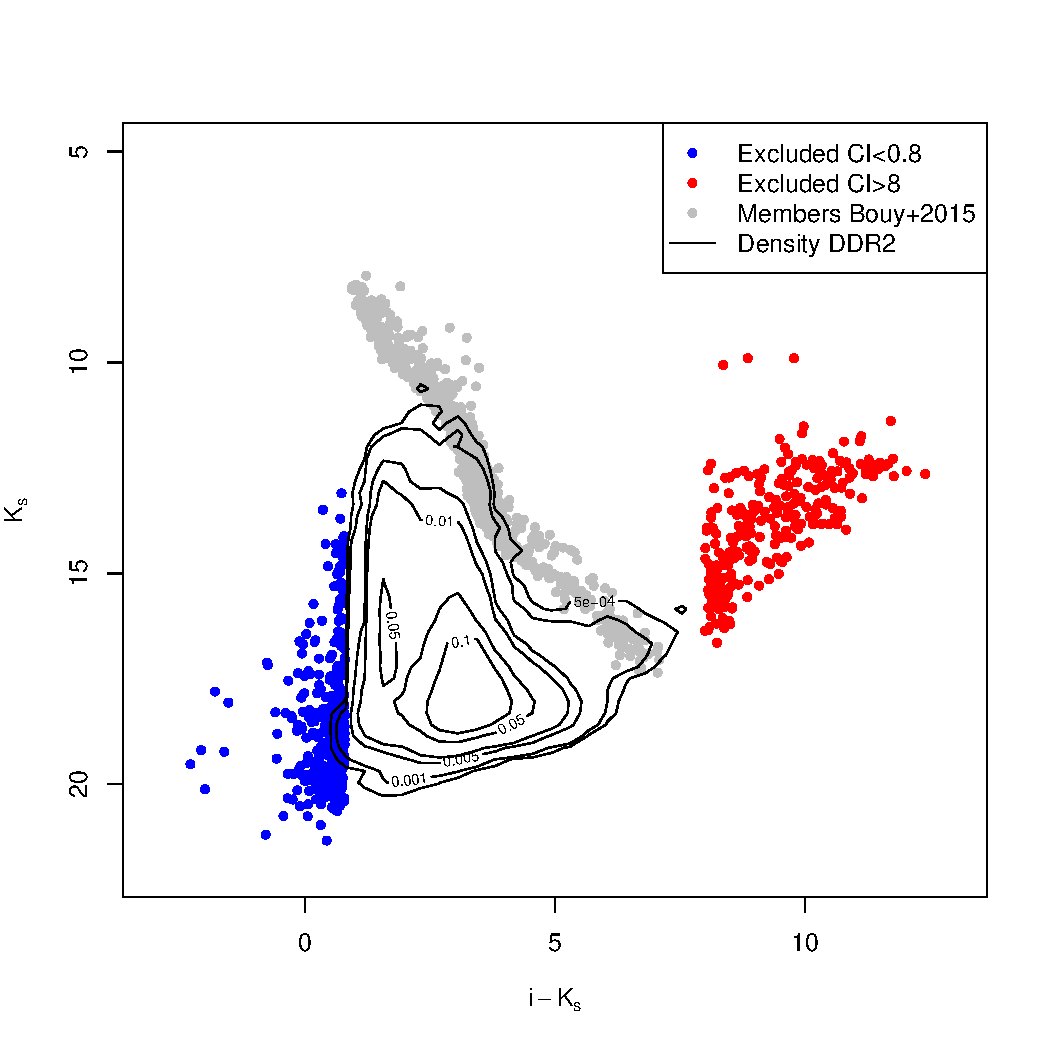
\includegraphics[width=\textwidth]{background/Figures/ColourCuts.pdf}
\caption{$K_s$ vs \gls{ci} \gls{cmd} showing the density (black contour lines) of all objects (with observed entries in this \gls{cmd}) in the \gls{ddr2}. Also shown, the candidate members of \citet{Bouy2015} (grey dots), and the objects excluded by the cuts at \gls{ci}=0.8 (blue dots) and \gls{ci}=8 (red dots). See text for details.}
\label{fig:incompatible_objects}
\end{center}
\end{figure}


With the previous restrictions to the \gls{ddr2} reduced it to 1 424 893 objects, with the largest number of rejected objects ($\sim 500\, 000$) resulting from a completely missing photometry.

\subsubsection{The Restricted DANCe Data Release 2 (RDDR2)}
Our computational constraints and the costly computations of our methodology (see Sect. \ref{sect:BHM}), prevented its application to the entire data set. However, since the precision of our methodology, as that of any statistical analysis, increases with the number of independent observations, we find that a size of $10^5$ source for our data is a reasonable compromise. Although a smaller data set produces faster results, it also renders a less precise and potentially more biased model of the field (in the area around the cluster) and therefore, a more contaminated model of the cluster. Thus, our data set was restricted to the $10^5$ objects with highest membership probabilities according to \citet{Bouy2015}. \textbf{This is equivalent to set a probability threshold at $p=1.05e^{-11}$ and select objects above this level.} In the following I refer to this data set as the \gls{rdr2}. The majority of these objects ($\sim$98\%) belong to the field with cluster membership probabilities about zero according to \citet{Sarro2014,Bouy2015}. Thus, under the assumption that the membership probabilities given by these authors are correct, the probability of leaving out a cluster member is negligible. The \gls{rdr2} data set is used to construct the cluster model and obtain the membership probability of its $10^5$ objects. For the remainder of the objects in the \gls{ddr2}, we assign membership probabilities \emph{a posteriori}, once the cluster model is constructed. 

Tables \ref{tab:rddr2_cluster} and \ref{tab:rddr2_field} show summaries of the observables and uncertainties for the 98012 field and 1988 cluster objects in the \gls{rdr2}, respectively. This classification is based on the membership probabilities and probability threshold ($p=0.75$) derived by \citet{Bouy2015}.

\begin{table}[ht!]
\caption{Summary of the 1988 candidate members of \citet{Bouy2015} in the \gls{ddr2}.}
\begin{center}
\begin{tabular}{|c|c|c|c|c|c|c|c|}
\hline
Observable & Min. & 1st. Qu. & Median & Mean & 3rd. Qu. & Max. & NA's \\
\hline
\hline
$\mu_{\alpha} [mas\cdot yr^{-1}]$&-81.64 &  14.45  & 16.24 &  16.30  & 18.14  & 90.32&0\\
$\mu_{\delta} [mas\cdot yr^{-1}]$&-81.88&  -42.09 & -39.85  & -39.62  &-37.45  & 82.59&0\\
i -$K_s$[mag] &  0.934 &   3.002 &  3.364  & 3.396 &  3.678 &  7.085  &   713\\
Y [mag]& 8.284 & 13.700 & 14.450  &14.690  &15.400 & 20.390  &   518\\
J [mag]& 6.545 & 11.950 & 13.400  &13.160 & 14.380  &19.310   &    6\\
H [mag]& 6.587 & 11.330 & 12.850  &12.610&  13.840 & 18.300   &   13\\
$K_s$ [mag]& 6.514 & 11.090 & 12.530 & 12.300 & 13.500 & 17.360   &    1\\
\hline
\multicolumn{8}{c}{Uncertainties}\\
\hline
Observable & Min. & 1st. Qu. & Median &Mean& 3rd. Qu. & Max. & NA's \\
\hline
\hline
$\mu_{\alpha} [mas\cdot yr^{-1}]$&0.08&0.25&0.76&0.5201&2.02&1e+5 &0\\ 
$\mu_{\delta} [mas\cdot yr^{-1}]$&0.08&0.25&0.76&0.52&2.02&1e+5& 0\\ 
i [mag] & 0.0200 & 0.0200 & 0.0200 & 0.0351 & 0.0202 & 2.1610&713 \\
Y [mag] & 0.0300&  0.0500&  0.0501&  0.0569&  0.0503 & 0.2392&518\\
J [mag] & 0.02000& 0.02700& 0.05005 &0.04270& 0.05014 &0.15990&6\\
H [mag] & 0.02000 &0.02700& 0.04009 &0.03994 &0.05010 & 0.14340&13\\
$K_s$[mag]&0.02000& 0.05003& 0.05045& 0.05278 &0.06001 &9.99500&1\\
\hline
\end{tabular}
\end{center}
\label{tab:rddr2_cluster}
\end{table}%

\begin{table}[ht!]
\caption{Summary of the 98012 filed objects in the \gls{rdr2}.}
\begin{center}
\begin{tabular}{|c|c|c|c|c|c|c|c|}
\hline
Observable & Min. & 1st. Qu. & Median & Mean & 3rd. Qu. & Max. & NA's \\
\hline
\hline
$\mu_{\alpha} [mas\cdot yr^{-1}]$&-99.980& -11.730  & 1.803 &  1.307 & 15.050 & 99.910&0\\
$\mu_{\delta} [mas\cdot yr^{-1}]$&-99.990& -17.980  &-4.820  &-4.088   &9.189  &99.980&0\\
i -$K_s$[mag] &   1.04 &   3.49  &  5.13    &   4.81  &  5.81  &  7.99 &  95628 \\
Y [mag]          & 9.97  & 18.70      &  19.45 &  18.83 &  19.93 &  22.23  & 21988 \\
J [mag]          & 3.954 & 17.790 & 18.660 & 17.880 & 19.160 & 20.620 &   7305\\
H [mag]         & 2.969 & 16.950 & 17.750 & 17.020 & 18.210 & 20.270  &  7655\\
$K_s$ [mag] & 2.598 & 16.260 & 16.960  &16.360  &17.370 & 21.020 &   5013\\
\hline
\multicolumn{8}{c}{Uncertainties}\\
\hline
Observable & Min. & 1st. Qu. & Median &Mean& 3rd. Qu. & Max. & NA's \\
\hline
\hline
$\mu_{\alpha} [mas\cdot yr^{-1}]$&0.08  &    8.65   &  14.94   &  23.50   &  25.60 &1.0e+05&0\\ 
$\mu_{\delta} [mas\cdot yr^{-1}]$&0.085  &   8.652  &  14.940  &  20.710  &  25.600 &1.86e+04 & 0\\ 
i [mag] & 0.02        &  0.02    &    0.07 &   0.08 &  0.12   & 0.66    &    95628 \\
Y [mag] & 0.030     &   0.068&   0.103&  0.112 &   0.148&0.938  &   21988\\
J [mag] & 0.020      &  0.065  & 0.097  & 0.104 & 0.136  &0.403   & 7305\\
H [mag] & 0.020     &  0.065  & 0.093  &0.099  & 0.124  &9.998   & 7655\\
$K_s$[mag]&0.020 &  0.060 &  0.079 & 0.087  & 0.101 & 9.998  & 5013\\
\hline
\end{tabular}
\end{center}
\label{tab:rddr2_field}
\end{table}%



\section{The Tycho+DANCe candidate members}
\label{sect:Tycho+DANCe}
Here I describe the data set used for the analysis of the Pleiades \gls{psd}. This data set is the largest and less contaminated list of Pleiades candidate members to date. It comprises, for the middle and faint luminosities, the \gls{hmps} of candidate members recovered by the \gls{bhm}, described in Section \ref{sect:memberscomparison}, and summarised in Table \ref{tab:hmps}, and for the high luminosities, the Tycho+DANCe candidate members of \cite{Bouy2015}, summarised in Table \ref{tab:tycho2}.

This joint data set comprises the positions in equatorial coordinates R.A. and Dec. (in the following $\alpha$ and $\delta$), proper motions, photometry, and membership probabilities of 2060 unique sources. 
However, for the analysis of the \gls{psd} we work only with the positions, membership probabilities, and $J$ photometric band. The latter is the bluest most available photometric band for this list of members. It will be used as a proxy for the mass, and to explore evidence of mass segregation.

\begin{table}[ht!]
\caption{Summary of the 1967 objects classified as members by the \gls{bhm}.}
\begin{center}
\begin{tabular}{|c|c|c|c|c|c|c|c|}
\hline
Observable & Min. & 1st. Qu. & Median & Mean & 3rd. Qu. & Max. & NA's \\
\hline
\hline
RA [deg]   & 51.42 &  55.67 & 56.69 &  56.76  & 57.81  & 62.81 & 0\\
Dec. [deg] &19.13  & 23.11  & 24.10 &  24.13  & 25.22 &  29.56 &0\\
$\mu_{\alpha} [mas\cdot yr^{-1}]$&-23.34  & 14.59  & 16.32 &  16.73 &  18.37  & 53.84&0\\
$\mu_{\delta} [mas\cdot yr^{-1}]$&-81.370 &-42.410& -40.130& -40.480& -37.760&  -2.016&0\\
i -$K_s$[mag] &  0.934 &  2.979  & 3.357    & 3.325   &  3.648  &6.662   &643\\
Y [mag]           &   8.284 & 13.660 & 14.360  &14.590  &15.310  &20.100 &   467 \\
J [mag]           &   7.058 & 12.060& 13.370  & 13.180 & 14.290 & 18.570&      5\\
H [mag]          &   7.009 & 11.430 & 12.810  & 12.620 & 13.750 & 17.480&      9 \\
$K_s$ [mag]  &   7.008 & 11.190 & 12.500  & 12.320 & 13.410 & 16.740&    0\\
\hline
\end{tabular}
\end{center}
\label{tab:hmps}
\end{table}%

\begin{table}[ht!]
\caption{Summary of the 207 objects from the Tycho2+DANCe data set classified as Pleiades candidate members ($P>0.48)$ by \citet{Bouy2015}.}
\begin{center}
\begin{tabular}{|c|c|c|c|c|c|c|c|}
\hline
Observable & Min. & 1st. Qu. & Median & Mean & 3rd. Qu. & Max. & NA's \\
\hline
\hline
RA [$^\circ$]                                 				            &  52.05&55.89 & 56.46 &56.55  &57.30   &  62.49  & 0\\
Dec. [$^\circ$]                       					           &  18.56&23.13  & 24.08& 23.99  &24.88  & 29.89 &0\\
$\mu_{\alpha} [\mathrm{mas}\cdot \mathrm{yr}^{-1}]$   &      9.7 &18.9   & 20.1  &    20.0 &  21.1   &  26.7&0\\
$\mu_{\delta} [\mathrm{mas}\cdot \mathrm{yr}^{-1}]]$   &  -55.10&-46.60&-45.10&-45.19 &-43.70  & -37.70&0\\
i [mag]								            &   7.910&9.321 & 10.21&  10.04 &   10.76& 12.960&   72\\
J [mag]          								    &   3.800& 7.588& 8.638& 8.451 & 9.575  &10.590&      0\\
H [mag]        								    &   3.864& 7.535& 8.463& 8.236 & 9.209  & 10.030&      0 \\
$K_s$ [mag]  							            &   3.879&7.478 & 8.373& 8.167  &  9.113 &  9.929&    0\\
\hline
\end{tabular}
\end{center}
\label{tab:tycho2}
\end{table}%

\subsection{Contamination and completeness}
\label{sect:TDContamination}
In Section \ref{sect:classifier}, we estimate a contamination rate of $4.3\pm0.2$\% in the \gls{hmps}, which
would amount to 84 of the 1967 candidate members. Also, \citet{Sarro2014} estimate that the contamination rate of their methodology is $11.0\pm2.0$\% for a probability threshold of $p=0.5$, as the one used by \citet{Bouy2015} to classify the candidate members of their Tycho+DANCe data set.  Thus, in our combined Tycho+DANCe list of candidate members, we acknowledge a mean contamination rate of $\sim 8\%$. We would expect these contaminating sources to be uniformly distributed in right ascension and declination because the position on the sky was explicitly removed from the calculation of membership probabilities.

We estimate the completeness of our list of candidate members, in terms of the J band luminosity and
spatial coverage, by assessing the completeness of the joint Tycho+DANCe survey. In Fig. \ref{fig:completeness} we show the distribution of the number of sources in the combined DANCe+Tycho catalogue as a function of the radial position for different limiting magnitudes in the J band.
The radial position is computed assuming a distance of 134.4 pc to the Pleiades cluster \citep{Galli2017} and a centre at $\alpha,\delta =[56.65,24.13]$. Distances are corrected by geometric distortions of large angles (using Eqs. \ref{eq:distfree} and \ref{eq:rs_and_ts}).
As can be seen from this figure, the DANCe+Tycho catalogue is complete until magnitude $J\sim19$ and radial distance of 11.5 pc ($\sim5^\circ$). We notice that the latter corresponds roughly with the sky coverage of the UKIDSS survey \citep{2007MNRAS.379.1599L}.
Hence, we restrict our list of candidate members to those with: i) J band observed and less than 19 mag., and ii) radial distances less than 11.5 pc. This results in 1964 candidate members, which represents more than 50\% more candidate members that those of  \citet{Converse2010}, who did the latest analysis of the Pleiades PSD.

Nevertheless, we remind the reader that the inhomogeneities (e.g. spatial resolutions, gaps in luminosity) of the data DANCe+Tycho data set are so complex (and some of them only partially understood) that can indeed bias the sample of candidate members in unknown ways. For example, the gap in luminosity coverage between the faint end of Tycho-2 catalogue and the bright end of the DANCe survey (see in Fig. 8 of \citealt{Bouy2015}) may result in undetected sources, therefore unmeasured proper motions and finally an incomplete list of candidate members.

\begin{figure}[ht!]
\begin{center}
\includegraphics[page=2,width=\columnwidth]{./background/Figures/RadiiDistribution_Tycho+DANCe_Jmag.pdf}
\caption{Density of sources in the combined DANCe+Tycho catalogue as a function of the radial distance to the cluster centre and limiting magnitude in the J band. The vertical grey line marks the limit of spatial completeness, 11.5 pc.}
\label{fig:completeness}
\end{center}
\end{figure}




